
%%%%%%%%%%%%%%%%%%%%%%%%%%% asme2e.tex %%%%%%%%%%%%%%%%%%%%%%%%%%%%%%%
% Template for producing ASME-format articles using LaTeX            %
% Written by   Harry H. Cheng                                        %
%              Integration Engineering Laboratory                    %
%              Department of Mechanical and Aeronautical Engineering %
%              University of California                              %
%              Davis, CA 95616                                       %
%              Tel: (530) 752-5020 (office)                          %
%                   (530) 752-1028 (lab)                             %
%              Fax: (530) 752-4158                                   %
%              Email: hhcheng@ucdavis.edu                            %
%              WWW:   http://iel.ucdavis.edu/people/cheng.html       %
%              May 7, 1994                                           %
% Modified: February 16, 2001 by Harry H. Cheng                      %
% Modified: January  01, 2003 by Geoffrey R. Shiflett                %
% Modified: September 3, 2008 by Matthew Millard                     %
% Use at your own risk, send complaints to /dev/null                 %
%%%%%%%%%%%%%%%%%%%%%%%%%%%%%%%%%%%%%%%%%%%%%%%%%%%%%%%%%%%%%%%%%%%%%%

%%% use twocolumn and 10pt options with the asme2e format
%\documentclass[twocolumn,10pt]{asme2e}
\documentclass[singlecolumn,12pt]{article}


\usepackage{amsmath, amssymb}
\usepackage[pdftex]{graphicx}
\usepackage{setspace}
\usepackage{times}
\usepackage{epsfig}
\usepackage{graphicx}
\usepackage{amsmath}
\usepackage{amssymb}
\usepackage{lscape}
\usepackage[top=1in, left=1.0in, right=1.0in, height=9in]{geometry}
\usepackage{fancyhdr}
\pagestyle{fancy}

\usepackage{color}
\usepackage{alltt}
\newcommand{\hlstd}[1]{\textcolor[rgb]{0,0,0}{#1}}
\newcommand{\hlkey}[1]{\textcolor[rgb]{0,0,1}{\bf{#1}}}
\newcommand{\hlnum}[1]{\textcolor[rgb]{0.66,0,0.66}{#1}}
\newcommand{\hltyp}[1]{\textcolor[rgb]{0,0,1}{#1}}
\newcommand{\hlesc}[1]{\textcolor[rgb]{0.77,0.18,0.66}{#1}}
\newcommand{\hlstr}[1]{\textcolor[rgb]{1,0,0}{#1}}
\newcommand{\hldstr}[1]{\textcolor[rgb]{1,0,0}{#1}}
\newcommand{\hlcom}[1]{\textcolor[rgb]{0.4,0.4,0.4}{\it{#1}}}
\newcommand{\hldir}[1]{\textcolor[rgb]{0,0.72,0}{#1}}
\newcommand{\hlsym}[1]{\textcolor[rgb]{1,0,0}{#1}}
\newcommand{\hlline}[1]{\textcolor[rgb]{0.4,0.4,0.4}{#1}}

\lhead{} \chead{Solvere4D Manual} \rhead{}

\lfoot{} \cfoot{p. \thepage} \rfoot{}
% Include other packages here, before hyperref.

% If you comment hyperref and then uncomment it, you should delete
% egpaper.aux before re-running latex.  (Or just hit 'q' on the first latex
% run, let it finish, and you should be clear).
\usepackage[pagebackref=true,breaklinks=true,letterpaper=true,colorlinks=false,bookmarks=false]{hyperref}
%\usepackage{lineno}

\def\httilde{\mbox{\tt\raisebox{-.5ex}{\symbol{126}}}}
\renewcommand{\baselinestretch}{1.0}

%\usepackage{times}

%% The class has several options
%  onecolumn/twocolumn - format for one or two columns per page
%  10pt/11pt/12pt - use 10, 11, or 12 point font
%  oneside/twoside - format for oneside/twosided printing
%  final/draft - format for final/draft copy
%  cleanfoot - take out copyright info in footer leave page number
%  cleanhead - take out the conference banner on the title page
%  titlepage/notitlepage - put in titlepage or leave out titlepage
%
%% The default is oneside, onecolumn, 10pt, final

%%% Replace here with information related to your conference
%\confshortname{IDETC/CIE 2007}

%----------------------------------------------------------------------
%\confshortname{the ASME 2007}
%\conffullname{International Design Engineering Technical Conferences \&\\
              % Computers and Information in Engineering Conference \\
              % IDETC/CIE 2007}

%\confdate{4-7}
%\confmonth{September}
%\confyear{2007}
%\confcity{Las Vegas, Nevada}
%\confcountry{USA}

%----------------------------------------------------------------------
%%% Replace DETC2005-12345 with the number supplied to you
%%% by ASME for your paper.

% \papernum{DRAFT \hskip 30mm DETC2007-35351}



\begin{document}

%%%%%%%%% TITLE
\title{Solvere 4D Multibody Dynamics \\ Post-processor Manual}

\author{Matthew Millard\\
University of Waterloo\\
 200 University Ave West\\
Waterloo ON, N2L 3G1, Canada\\
{\tt\small mjhmilla@engmail.uwaterloo.ca}}



% For a paper whose authors are all at the same institution,
% omit the following lines up until the closing ``}''.
% Additional authors and addresses can be added with ``\and'',
% just like the second author.
% To save space, use either the email address or home page, not both


\maketitle
% \thispagestyle{empty}

\begin{figure}[!h]
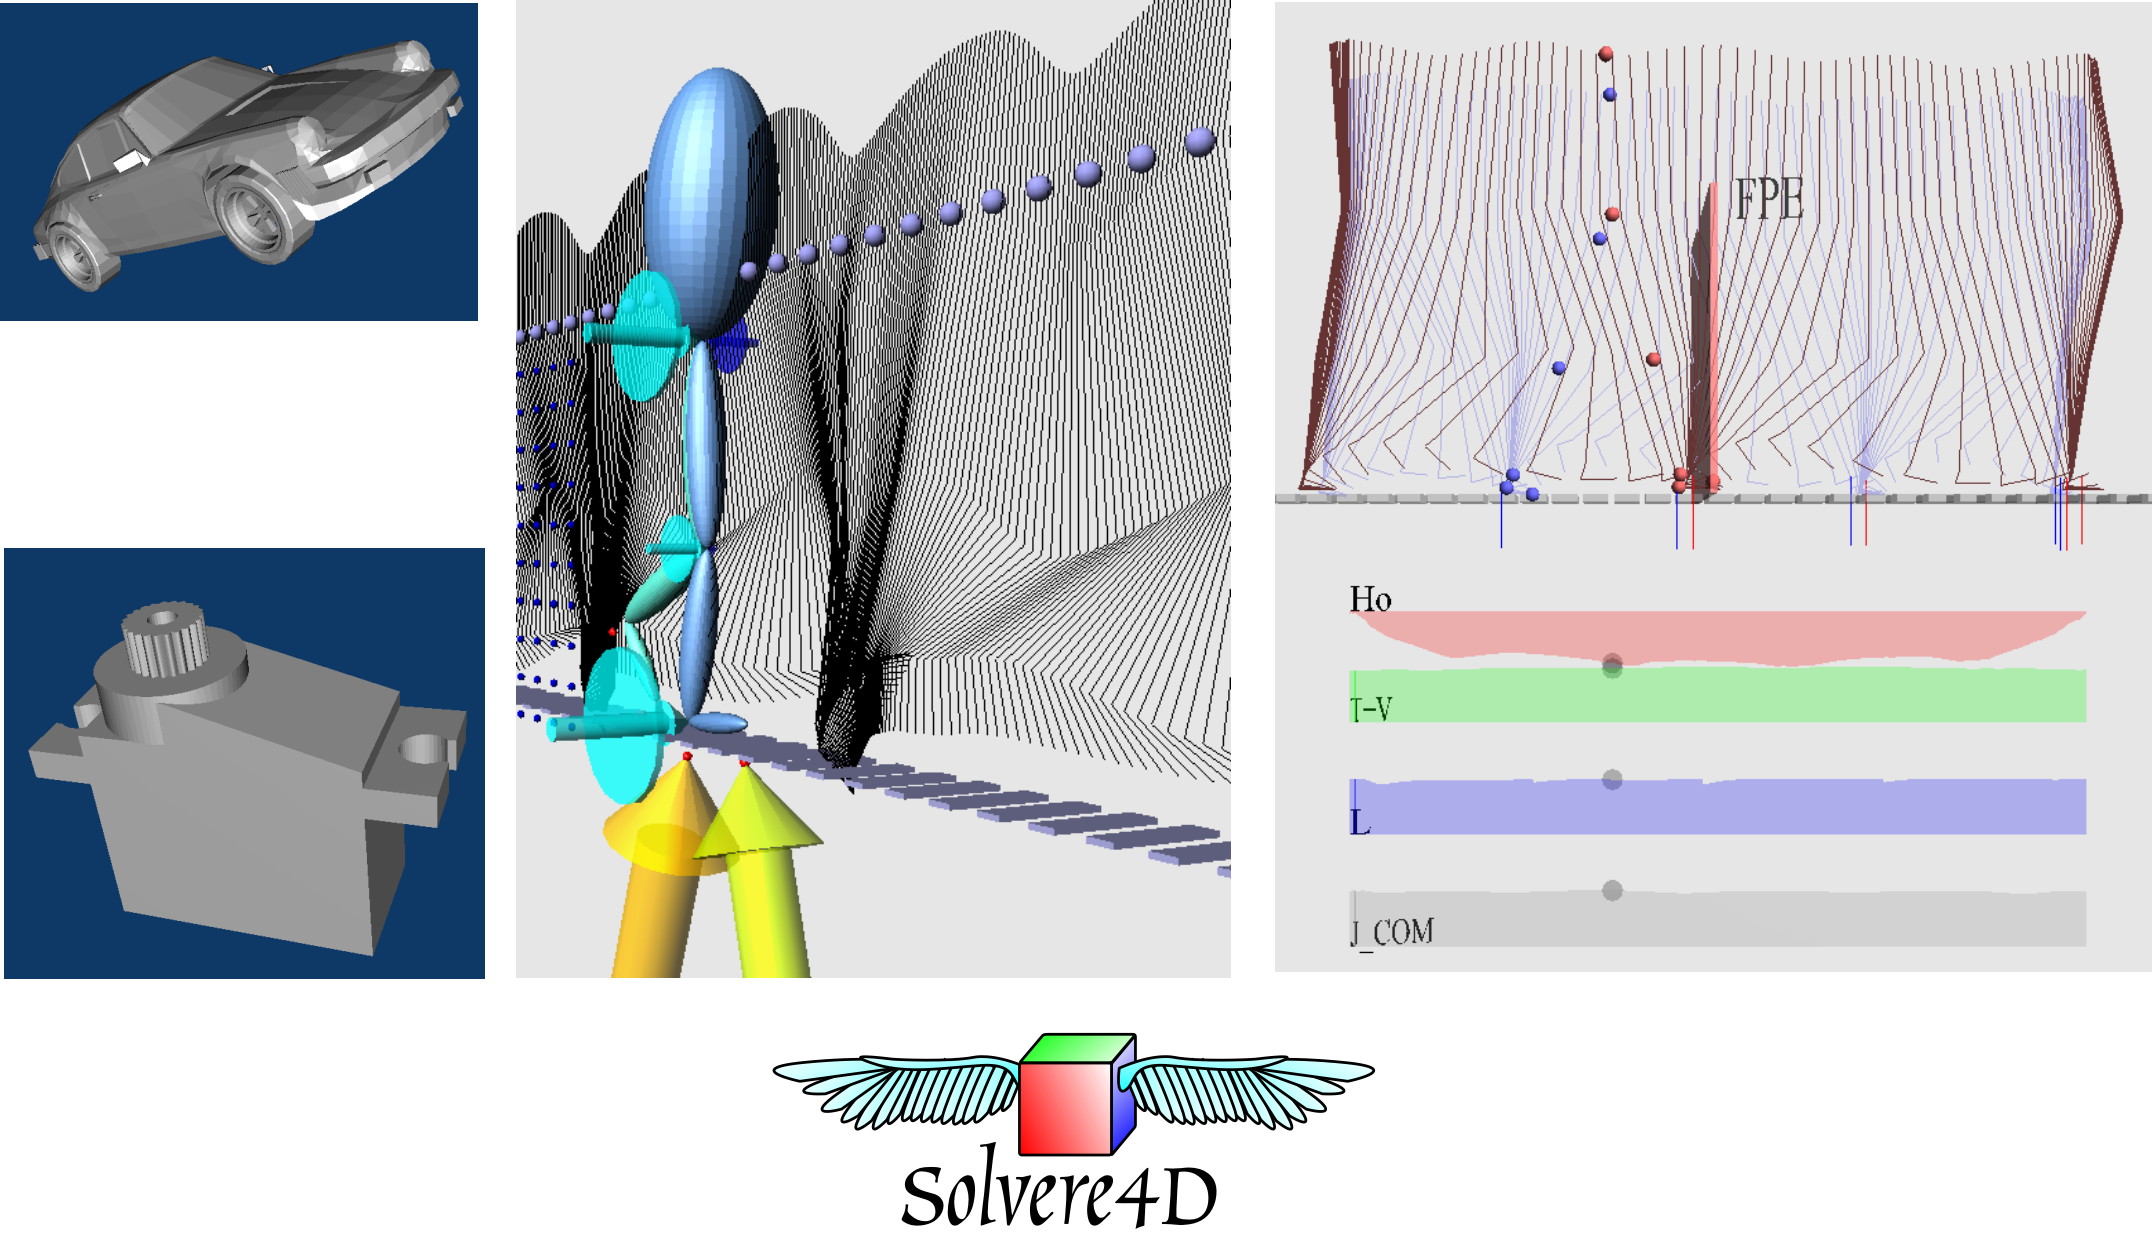
\includegraphics[width = \textwidth, height = \textheight, keepaspectratio= true]{fig_splash}
\end{figure}


%%%%%%%%% ABSTRACT
\newpage
\begin{abstract}
Solvere4D is a powerful, open-source, freely available
post-processor that makes it easy for anyone to generate 3D
animations of their data. Solvere4D is particularly designed for
people who are in multibody dynamics, or kinesiology. Solvere4D can
help you easily create intuitive research-grade 3D animations that
include integrated plotting, force/torque visualization and
graphical kinetic and kinematic history displays to enhance the
insight gained from your data. Play back controls are embedded to
allow you to play/pause the animation, speed or slow the rate of
play back and randomly access different times in the animation using
a slider. Solvere4D also includes powerful command-line tools that
allow you to automate the creation of your 3D animations. With
Solvere4D you can quickly and efficiently generate animations that
allow you to see the equivalent of 20 or more data plots in one
intuitive animation. ``Solvere" is Latin for ``to free" or ``to
release", accordingly Solvere4D is offered as free, open-source
software under the GNU GPL Licence. This means to you can learn how
Solvere4D works and add your own code to it to improve it.
\end{abstract}

\newpage
\tableofcontents

%%%%%%%%% BODY TEXT
\newpage
\section{Introduction}
\label{sec_Intro}

\begin{figure}[!h]
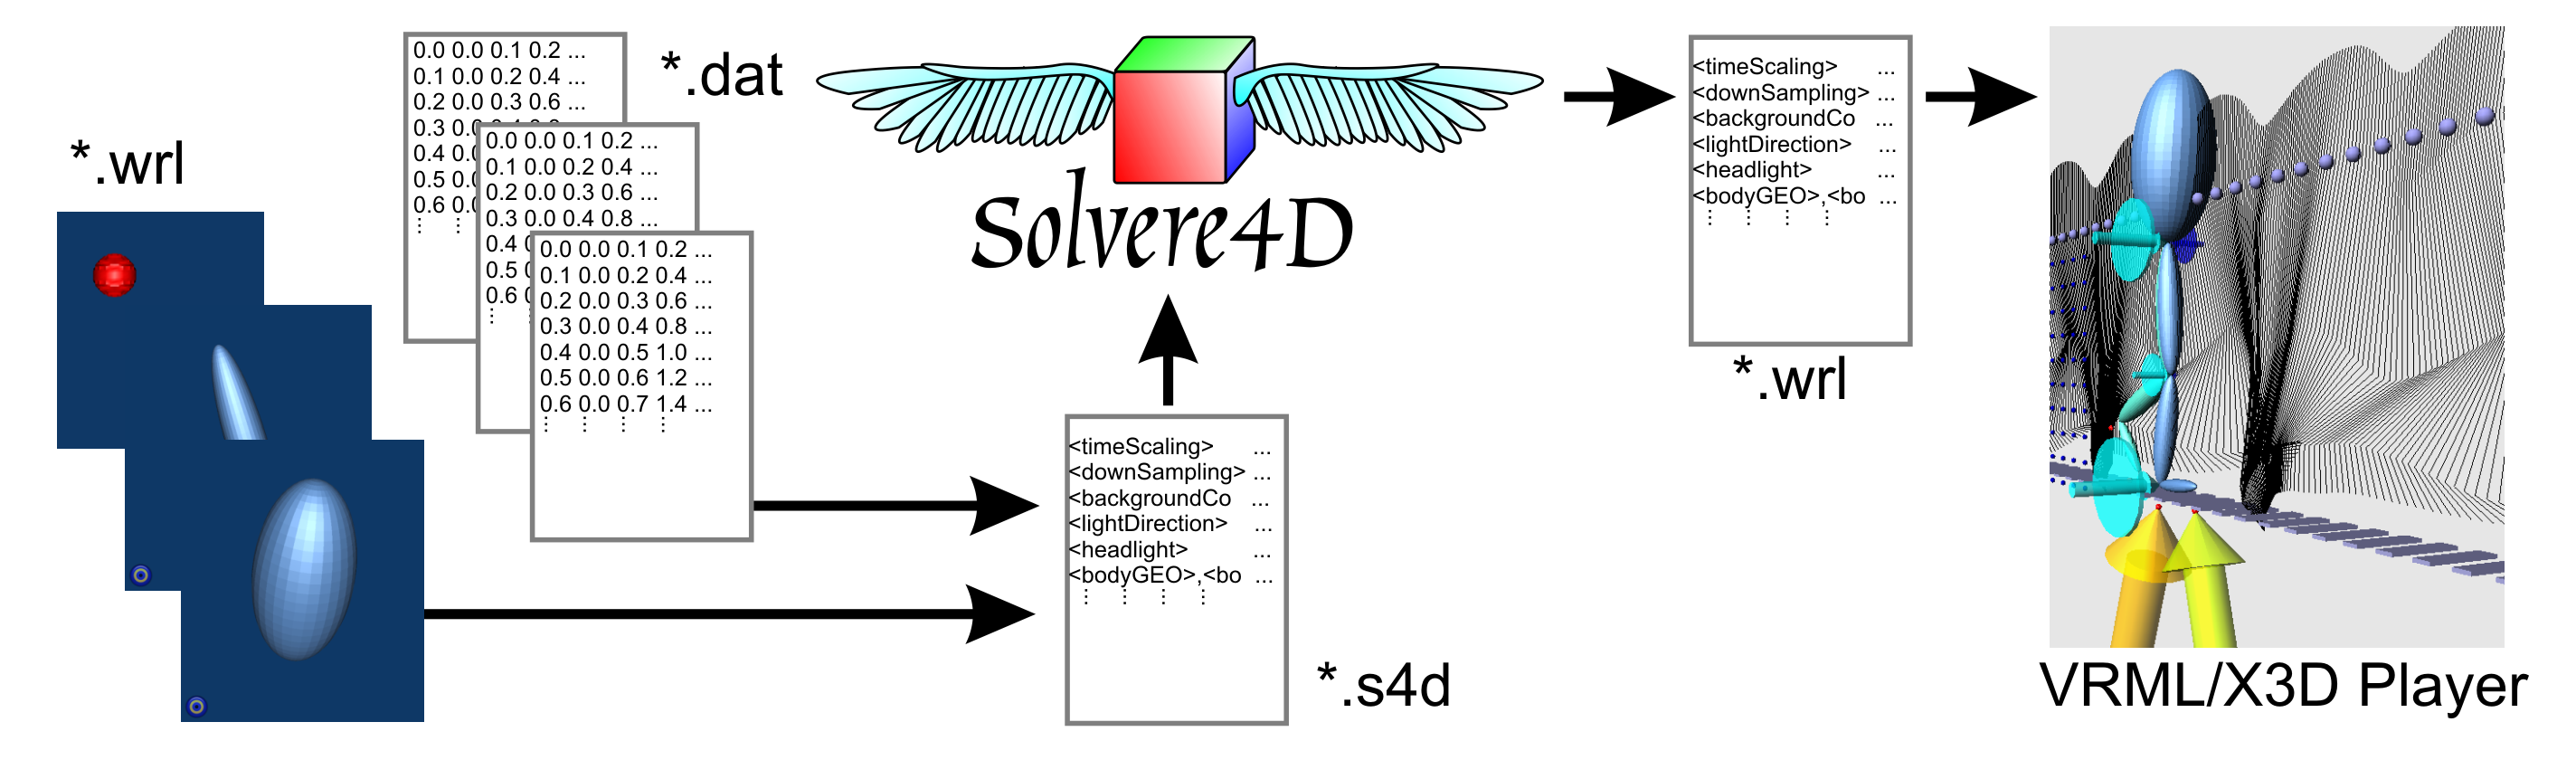
\includegraphics[width = \textwidth, height = \textheight, keepaspectratio= true]{fig_solvere_system}
\caption{Solvere takes data files (*.dat), geometry files (*.wrl) a
configuration file (*.s4d) and turns it into a 3D animation file
(*.wrl). This animation file can be viewed using a number of
different VRML/X3D players.\label{fig_solvere_system}}
\end{figure}

Solvere4D will take your exported data, body geometry, a
configuration file and turn it into a 3D animation file as shown in
Fig. \ref{fig_solvere_system}. This animation file can then be
played by any number of different VRML/X3D viewers. The remainder of
this section will describe how to run Solvere4D and how to view 3D
VRML movies. Section \ref{sec_writingConfigFiles} onwards will
describe how to use all of Solvere4D's features and how to
contribute to Solvere4D.

\subsection{Playing VRML/X3D Files}

Solvere4D creates 3D animation files, or Virtual Reality Markup
Language (VRML) files. These files on their own are not useful, but
they contain commands that a VRML/X3D viewer can translate into 3D
animations. There are many different VRML viewers available to you:

\vspace{1cm}
\begin{tabular}{l | l | l | l}
Software & Windows & Linux & Mac \\
\hline Cosmo Player & X & & \\
BSContact & X & X & \\
BS Contact J & X & X & X \\
Octaga Player & X & X & X \\
InstantPlayer & X & X & X \\
Cortona3D & X & & X \\
Vivaty Player & X & & \\
SwirlX3D & X & & \\
FreeWRL & & X & X \\
OpenVRML & & X & X \\
Xj3D & X & X & X  \\
Orbisnap & X & X & X \\
Demotride & X & & \\
\end{tabular}
\vspace{1cm}

The preceding list can be found with hyper-links to each program at
\url{http://cic.nist.gov/vrml/vbdetect.html}. I have tried out
BSContact, Octaga, InstantPlayer, Cortona3D, SwirlX3D and FreeWRL.
The best player by far is BSContact's player for the Windows
platform, next I would recommend Octaga. The main difference between
the players is how much of the VRML specification they implement.
Some will not display text making it impossible to view the
animations current time among other things. Some will not implement
a ``touchSensor" node, making it impossible to press the
``Play/Pause", ``Slow Down/Speed up" buttons.

If you cannot use BSContact it may take you some time to find a good
VRML viewer. Once you do have a good VRML viewer you can look at the
3D world for the first time:

\begin{enumerate}
\item Open ``Examples/experimental\_data/fpe\_research.wrl".
\item Use the controls pictured in Fig.
\ref{fig_timecontrols_detail} to run the animation:

\begin{itemize}
\item Play/Pause: Press the blue button. By default the animation is
paused to begin. You may need to click on the screen above the time
controls before clicking the blue button to start.
\item Increase rate of play: Press the up triangle
\item Decrease rate of play: Press the down triangle
\item Set the current animation time: Click and drag on the grey
time pointer that runs along the time slider
\item Note: the rate of play is displayed on the left of the
display, while the current animation time is displayed in
hours:minutes:seconds:milliseconds format.
\end{itemize}

\item Navigate around in the world:

\begin{itemize}
\item Use the arrow keys to move forward/backwards and look
left/right
\item Try using the other navigation methods to move around. The
viewer should have a way of changing the navigation mode
(right-click, then select the ``Movement" menu in BSContact). There
are several different modes available in VRML worlds:

\begin{enumerate}
\item Walk
\item Slide
\item Examine
\item Fly
\item Pan
\item Game-like
\end{enumerate}

Try all of them to see what they do, and what kinds of movement they
afford.

\end{itemize}

\item Open ``Examples/simulation\_data/airWalkHat.wrl" and run it to
see force and torque vector animations, and an animation that
involves more camera movement.

\end{enumerate}

\begin{center}
\begin{figure}[!h]
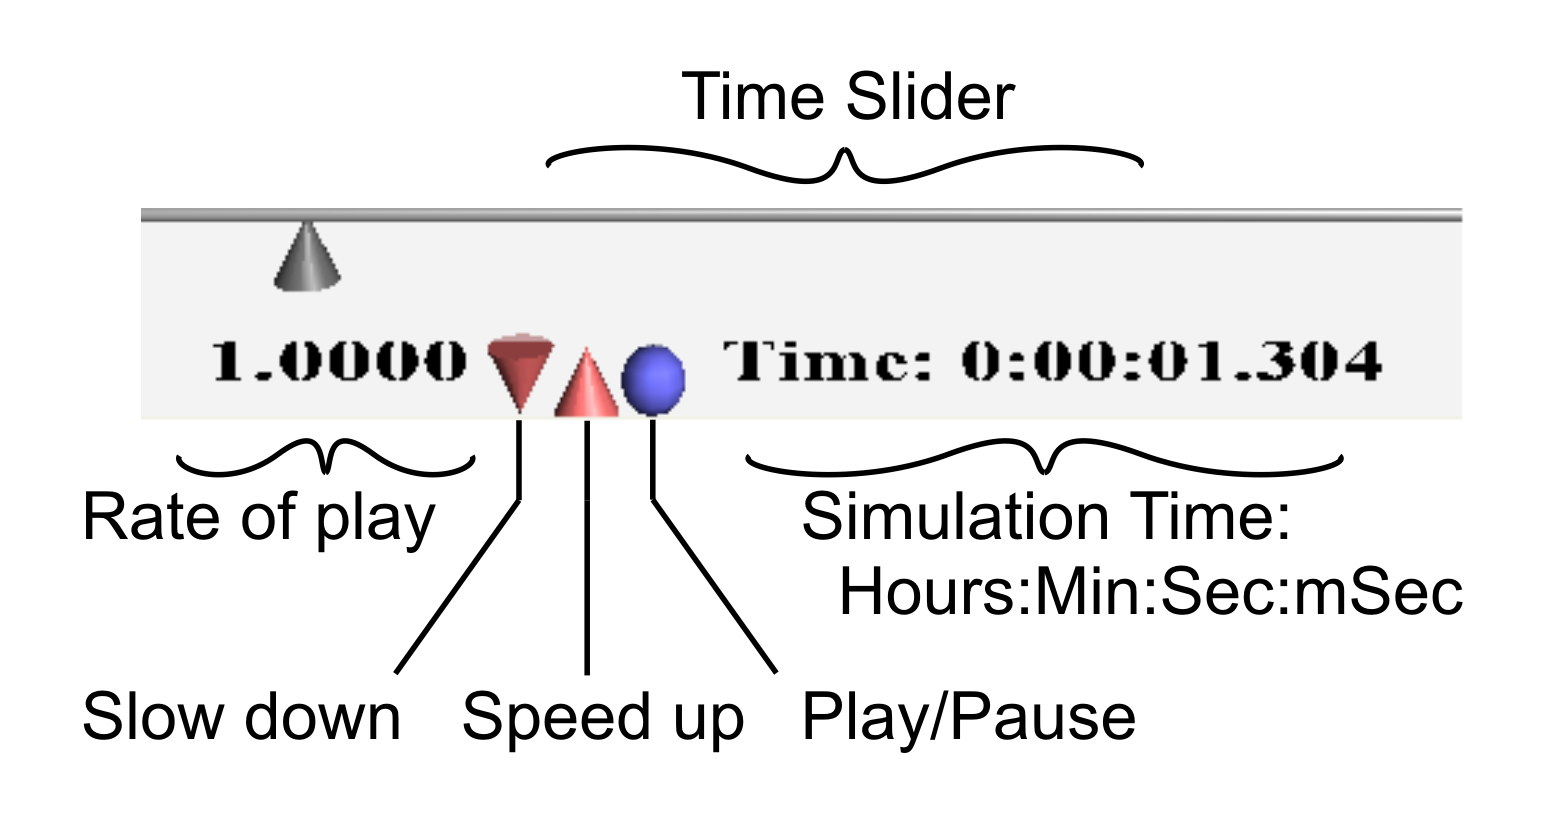
\includegraphics[width = 0.75\textwidth, height = 0.75\textheight, keepaspectratio= true]{fig_timecontrols_detail}
\caption{The animation can be played/paused, the rate of play
adjusted (sped up and slowed down) and the current animation time
can be manually adjusted using the controls that Solvere4D adds to
the animation.\label{fig_timecontrols_detail}}
\end{figure}
\end{center}

\subsection{Running Solvere4D}

Solvere4D can be run in two ways:

\begin{enumerate}
\item \textbf{GUI:} Double clicking ``runAnimation.bat" on a Windows machine
will launch the GUI. If you are not using windows, open up the *.bat
file and make the necessary syntax adjustments to run it on your OS.


\item \textbf{Command-line:} Issuing a "java Solvere4D.Solvere4D
C:/full/path/to/configfile/test.s4d" from within Solvere4D's
``build/classes" directory will cause Solvere4D to read the
specified
*.s4d configuration file and create an animation titled "test.wrl"
in the same directory as the *.s4d file.
\end{enumerate}

\begin{center}
\begin{figure}[!h]
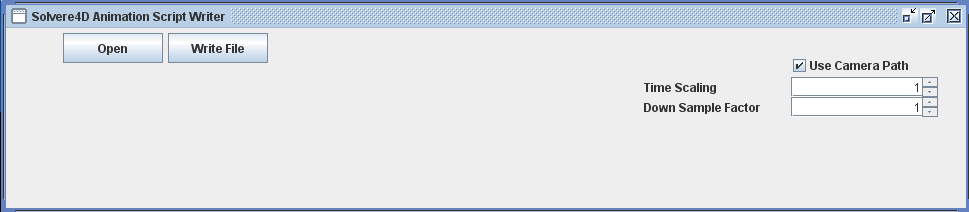
\includegraphics[width = 0.75\textwidth, height = 0.75\textheight, keepaspectratio= true]{fig_solvere4D_gui}
\caption{Solvere4D simple GUI. Some basic parameters like the time
scale, down-sampling and the choice of using the camera path can be
chosen here. Pressing the `Write File' button will cause Solvere4D
to write a 3D animation file (*.wrl) to the same directory that the
 configuration (*.s4d) file resides in.\label{fig_solvere4D_gui}}
\end{figure}
\end{center}

You should try launching Solvere4D's GUI, and using it to write a
VRML file using the steps below. A screen shot of the simple GUI is
shown in Fig. \ref{fig_solvere4D_gui}.

\begin{enumerate}
\item Double click the ``runAnimation.bat" file
\item Use the ``Open File" dialogue to navigate to the
``Manual/Examples/experimental\_data" folder and choose the
``fpe\_research.s4d" file.
\item Press the ``Write File" button
\item Go to the ``Manual/Examples/experimental\_data" folder and
look at the ``fpe\_research.wrl" files timestamp: it should be from
just a minute or two ago. View the *.wrl file using your VRML viewer
of choice
\end{enumerate}

You should also try to run Solvere4D from the command line. This is
a particularly useful skill to learn because you can use other
programs such as Matlab to run Solvere4D as detailed in Appendix
\ref{app_matlab}. This can allow you to completely automate the
production of 3D visualizations of your data. I have used this
technique to generate 1480 3D videos of experimental data (similar
to the ``fpe\_research.wrl" files) using Matlab and Solvere4D in the
span of a few hours. To run Solvere4D from the command line simply
follow these steps:

\begin{enumerate}
\item Open a command shell. A command shell can also be called a command prompt,
terminal or window in case you have not heard the term `shell'. In Windows follow these steps
\begin{enumerate}
\item Press ``Start"
\item Select ``Run"
\item Type ``cmd" in the little window
\item Press ``OK"
\end{enumerate}

\item Move the command shell to Solvere4D's ``build/classes" folder.
In Windows use the following steps:
\begin{enumerate}
\item Open a Windows folder
\item Navigate to Solvere4D's ``build/classes" folder
\item Select the text in the ``Address" bar and press "Ctrl C" to
copy it
\item In the command prompt type the text ``cd ", which stands for
``change directory"
\item Use the mouse to put the cursor after the ``cd " in the
command shell, then use the mouse to right-click. A menu will pop
up, select ``Paste". This should put your whole address in the line.
\item Press ``Enter". For example:


\footnotesize
\begin{verbatim}
cd C:\Solvere4D\build\classes
\end{verbatim}
\normalsize


\end{enumerate}

\item In the command shell type the text

\footnotesize
\begin{verbatim}
java Solvere4D.Solvere4D
\end{verbatim}
\normalsize

\item If you press ``Enter" now, you will launch the GUI. You'd
rather learn to use the script, so get the full path to you *.s4D
file and paste it in. For example

\footnotesize
\begin{verbatim}
java Solvere4D.Solvere4D C:\Solvere4D\Manual\Examples\experimental_data
\end{verbatim}
\normalsize


\item Add a slash and the name of the *.s4d configuration file. For
example:


\footnotesize
\begin{verbatim}
java Solvere4D.Solvere4D
"C:\Solvere4D\Manual\Examples\experimental_data\ fpe_research.s4d"
\end{verbatim}
\normalsize

The carriage-return should be ignored above, as this text should be
on one line in the command shell.


\item Now press enter. If all goes well the text below will pop up,
and one or two seconds later your new *.wrl file will be created and
ready to use.

\footnotesize
\begin{verbatim}
Copyright Matthew J.H.Millard 2008
  Solvere4D is offered under the GPL V3
  for more information visit http://www.gnu.org/
\end{verbatim}
\normalsize


\end{enumerate}


\subsection{Generating Geometry Files}

Solvere4D needs VRML97 files containing 3D representations of the
bodies you wish to animate. If you have never drawn a 3D shape
before do not worry, it is not too difficult. Many 3D CAD packages
can generate these files, and a free 3D sculpting program known as
Blender export VRML97 \url{http://www.blender.org/}. If your CAD
package cannot write a VRML97 file it can probably export a *.stl
file. Blender can import *.stl files and then export a VRML97 file
for you.

For mere convenience it is worth knowing the commands to draw the
basic VRML primitives (sphere, cylinder, cone and box) for your own
use. All of the primitive shapes in VRML are drawn for you in
`Examples/primitive\_geometry' folder - open up the files in any
text editor to see how each of these shapes are specified. Note: all
units are in meters. Simple spheres were used to animate the
positions of optical markers on a person as shown in the
``fpe\_research.wrl" file --- even simple markers can be quite
effective at displaying motion.

As you produce more sophisticated geometry you will want to ensure
that the centroid of the *.wrl part is at the same location as it is
in your data --- else the part will be animated with the wrong
initial orientation or perhaps with an offset. The position of the
parts centroid can be edited in Blender or in the CAD package you
happen to be using.


\newpage
\section{Writing Solvere *.s4d Configuration Files}
\label{sec_writingConfigFiles}

The following subsections will explain in detail how to write the
*.s4d configuration file that Solvere4D requires to write a 3D
animation of your data. Solvere4D uses this configuration file and
the data files to animate your data. This configuration file points
Solvere4D to the files that hold the data you wish to animate as
well as telling Solvere4D how to display it. There are some general
rules about how these data files should be formatted in order for
Solvere4D to use them:

\begin{enumerate}
\item All data files should be in the same folder as the *.s4d
configuration file.
\item All data files must be tab delimited.
\item Every data file that includes time as the first column must
have the same time as every other file.
\end{enumerate}

\subsection{Pre-amble Tags}
\begin{tabular}{l l l}
\hline Tag & Arguments  & Description \\
\hline $<$timeScaling$>$  & $>0$ & This scales the simulation time. A scaling of 2.0\\
                        &      &  would turn a 10 sec animation into a 20 second \\
                        &       & animation.\\
                        & & \\
$<$downSampling$>$    & Integer $>0$ & The integer value here will down sample \textit{all}\\
            &                      & of the data you insert into the animation. A value \\
            &                      & of 1 will not downsample the data, a value of 2 will \\
            &                      & take every second point, 3 every $3^{rd}$ point, etc \ldots \\
            & & \\
$<$backgroundColour$>$ & R\# G\# B\#  & The values placed after the letters `R', `G', and `B'\\
            &  \#:0.0-1.0           & correspond to an colour in Red-Green-Blue colour \\
            &                       & space. Decimal values of range 0-1 are used here. \\
            &                       & See appendix for a short primer on the RGB\\
            &                       &  colour space.\\
            & & \\
$<$lightDirection$>$ & $<$X\# Y\# Z\#$>$ & If you would like a white light shone on your \\
                   &   \#:0.0-1.0   &  scene, include this followed by a vector direction.\\
                   &                & For example to shine a light along the X axis you \\
                   &                & would enter $<X1.0 Y0.0 Z0.0>$. \\
                   & & \\
$<$headlight$>$ & Integer: [0,1]      & A value of 0 will turn off the headlight,\\
                &                   &  a 1 will turn it on \\
\end{tabular}

\vspace{1cm}

 Examples of pre-amble tags for the *.s4d configuration
file can be found below and in Appendix \ref{app_ex_s4d_Files}.

\vspace{1cm}

\hlnum{\\
}\hlkey{$<$timeScaling$>$}\hlstd{,\hlstd{\ \ \ \ }}\hlnum{1.0\\
}\hlstd{}\hlkey{$<$downSampling$>$}\hlstd{,\hlstd{\ \ \ \ }}\hlnum{2\\
}\hlstd{}\hlkey{$<$backgroundColour$>$}\hlstd{,\hlstd{\ \ }}\hlkey{$<$R}\hlnum{0.90\ }\hlkey{G}\hlnum{0.90\ }\hlkey{B}\hlnum{0.90}\hlkey{$>$}\hlstd{\\
}\hlkey{$<$lightDirection$>$}\hlstd{,\ }\hlkey{$<$X}\hlnum{-0.5\ }\hlkey{Y}\hlnum{-0.5\ }\hlkey{Z}\hlnum{-1}\hlkey{$>$}\hlstd{\\
}\hlkey{$<$headlight$>$}\hlstd{,\ }\hlnum{0}

\vspace{1cm}

\subsection{$<$bodyGEO$>$,$<$bodiesMOV$>$: Kinematic Animation Tag}

This simple tag will take geometry that you would like to animate,
and move it through space in the manner you desire. Currently
Solvere4D only accepts VRML97/VRML 2.0 (but not VRML 1.0) files to
specify its geometry. Many 3D CAD packages can generate these files,
and a free 3D sculpting program known as Blender export VRML97
\url{http://www.blender.org/}. With a little work Solvere4D can be
upgraded to accept X3D files, which is the latest upgrade to VRML97.
For mere convenience it is worth knowing the commands to draw the
basic VRML primitives (sphere, cylinder, cone and box) for your own
use. All of the primitive shapes in VRML are drawn for you in
`Examples/primitive\_geometry' folder - open up the files in any
text editor to see how each of these shapes are specified. Note: all
units are in meters.

To make your geometry move, you must supply a text file that
contains the position and orientation information about your part.
The data file must be tab-delimited have the following format:

\vspace{1cm}
\begin{center}
\begin{tabular}{c|c|c|c|c|c|c|c|c|c|c|c|c|c|}
\hline Column & 1 & 2 & 3 & 4 & 5 & 6 & 7 & 8 & 9 & 10 & 11 & 12 & 13 \\
\hline & Time & X & Y & Z & r11 & r12 & r13 & r21 & r22 & r23 & r31
& r32 &
r33 \\
\end{tabular}
\end{center}
\vspace{1cm}

Where r11,r12,r13 \ldots r33, are the entries of a rotation matrix
entered row wise so that r12 refers to the entry in row 1, column 2.
An example of such a file can be found in the file
`Examples/simulation\_data/HatPosOrien.dat'. Typically this data is
generated by your simulation, or gathered from experiments.

Once your geometry text is ready, and the data file required to move
the part you need to make an entry in the *.s4d configuration file
so that Solvere4D can include it in the final animation. For
geometry filed called `redsphere.wrl' and a movement file called
`M1.dat', and another `M2.dat' the entry would look like this:

\vspace{1cm}
\hlkey{$<$bodyGEO$>$}\hlstd{,}\hlkey{$<$bodiesMOV$>$}\hlstd{\\
\hlstd{\ \ \ \ \ \ \ \ \ }redsphere.wrl,\hlstd{\ \ \ \ }M1.dat\\
\hlstd{\ \ \ \ \ \ \ \ \ }redsphere.wrl,\hlstd{\ \ \ \ }M2.dat\\
}\hlstd{\ \ \ \ \
}\hlkey{$<$$\backslash$bodyGEO$>$}\hlstd{,}\hlkey{$<$$\backslash$bodiesMOV$>$}
\vspace{1cm}

Any subsequent geometry and movement file pairs should be added on a
separate line as shown in Appendix \ref{app_ex_s4d_Files}.

\subsection{$<$forceTorque$>$,$<$genForceTorquePlots$>$: Force/Torque Animation Tag}

The animation of forces and torques is automatically done for you in
Solvere4D, you only need to provide the force and torque histories
in a file and decide how you would like them displayed. Force
vectors are drawn as an arrow and torques as an arrow with a disc
with colour being dictated by the orientation of the vector as shown
in Fig. \ref{fig_forcetorque}. Force and torque vectors have their
size scaled with the their respective magnitudes; it is up to you to
choose the scaling that is most appropriate for your data.

\begin{figure}[!h]
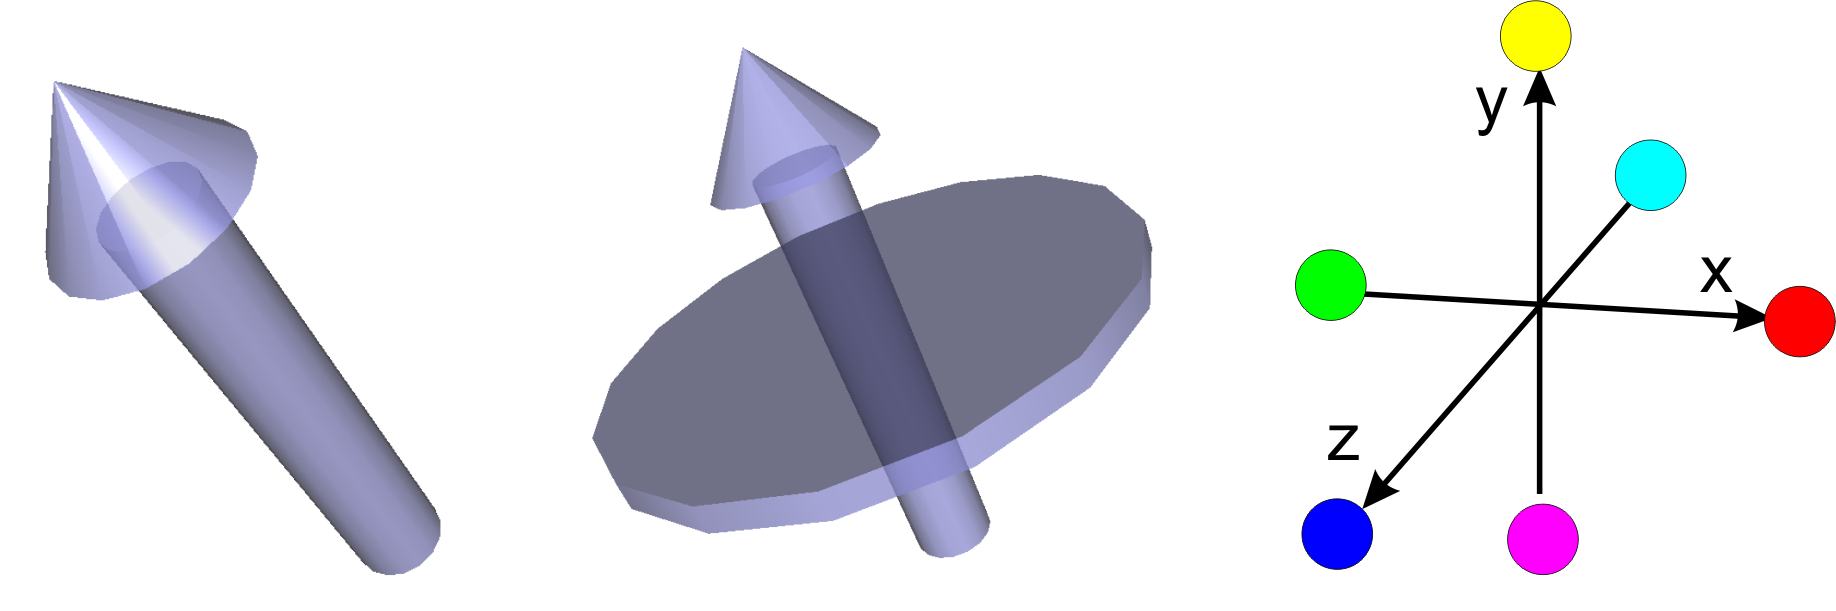
\includegraphics[width = \textwidth, height = \textheight, keepaspectratio= true]{fig_forcetorque}
\caption{Forces are represented with an arrow, torques as an arrow
with a disc. The colour of the vectors changes as a function of the
orientation - the colour of the major axis is shown above.
Orientations between the cardinal directions will have an
interpolated colour.\label{fig_forcetorque}}
\end{figure}

Forces and torques are loaded into Solvere4D using a tab delimited
file. The expected columns for the file are shown below.

\vspace{1cm}
\begin{center}
\begin{tabular}{c|c|c|c|c|c|c|c|c|c|c|}
\hline Column & 1 & 2 & 3 & 4 & 5 & 6 & 7 & 8 & 9 & 10 \\
\hline & Time & X & Y & Z & $F_X$ & $F_Y$ & $F_Z$ & $T_X$ & $T_Y$ & $T_Z$\\
\end{tabular}
\end{center}
\vspace{1cm}

Once your data file is ready, you need to tell Solvere4D how to
render your force/torque vectors using a series of statements. An
example of this is shown below:

\vspace{1cm}
\hlstd{\\
}\hlkey{$<$forceTorque$>$}\hlstd{,}\hlkey{$<$genForceTorquePlots$>$}\hlstd{\ normF=}\hlnum{1000.0\ }\hlstd{normT=}\hlnum{500.0\ }\hlstd{normD=}\hlnum{1.0\\
\hlstd{\ \ \ \ }}\hlstd{toeRightForces.dat,\hlstd{\ \ }}\hlkey{$<$f}\hlnum{0\ }\hlkey{w}\hlnum{0\ }\hlkey{c}\hlnum{0\ }\hlkey{R}\hlnum{0.0\ }\hlkey{G}\hlnum{0.0\ }\hlkey{B}\hlnum{0.5\ }\hlkey{T}\hlnum{0.5}\hlkey{$>$}\hlstd{\ }\hlkey{$<$t}\hlnum{0\ }\hlkey{w}\hlnum{1\ }\hlkey{c}\hlnum{1\ }\hlkey{R}\hlnum{1.0\ \ }\hlkey{G}\hlnum{0.5\ \ }\hlkey{B}\hlnum{0.0\ \ \ }\hlkey{T}\hlnum{0.5}\hlkey{$>$}\hlstd{\\
\hlstd{\ \ \ \ }heelRightForces.dat,\ }\hlkey{$<$f}\hlnum{0\ }\hlkey{w}\hlnum{0\ }\hlkey{c}\hlnum{0\ }\hlkey{R}\hlnum{0.0\ }\hlkey{G}\hlnum{0.0\ }\hlkey{B}\hlnum{1.0\ }\hlkey{T}\hlnum{0.5}\hlkey{$>$}\hlstd{\ }\hlkey{$<$t}\hlnum{0\ }\hlkey{w}\hlnum{1\ }\hlkey{c}\hlnum{1\ }\hlkey{R}\hlnum{0.0\ \ }\hlkey{G}\hlnum{0.5\ \ }\hlkey{B\ }\hlnum{1.0\ \ \ }\hlkey{T}\hlnum{0.5}\hlkey{$>$}\hlstd{\\
}\hlkey{$<$$\backslash$forceTorque$>$}\hlstd{,}\hlkey{$<$$\backslash$genForcePlots$>$}\hlstd{,}\hlkey{$<$$\backslash$genTorquePlots$>$}
\vspace{1cm}

The very first line contains the settings that control how the
forces entered in the *.dat file are turned into size
representations:

\vspace{1cm}
\begin{tabular}{l l l}
\hline Setting & Arguments  & Description \\
\hline normF= & \# $>$ 0 & All force vectors will be normalized using the\\
    &           & value entered in normF\\
normT= & \# $>$ 0 & All torque vectors will be normalized using the\\
    &           & value entered in normT\\
normD= & \# $>$ 0 & The normalized versions of the force and torque\\
        &       & vectors will be multiplied by normD in order to\\
        &       & set the vectors final size
\end{tabular}
\vspace{1cm}

 If you look at the example above you will note that the
forces are scaled such that a 1m long vector represents a force of
1000 N, and a torque vector with a 1m diameter disk would have a
torque of 500 Nm. Note that Solvere4D does not care about the units,
they were used in the previous sentence for clarity only.

In addition to simply rendering the force and torque vectors, you
can have a persistent 3D plot of the force and torque vectors drawn
in your animation. When used sparingly, this feature can be very
useful for examining the time history of the forces and torques in
more detail than is possible with the animation alone. The tags
following the file entry control way in which the force/torque
histories are displayed. For example, the tags that control how the
force/histories are displayed for the first file are:

\vspace{1cm} \hlkey{$<$f}\hlnum{0\ }\hlkey{w}\hlnum{0\
}\hlkey{c}\hlnum{0\ }\hlkey{R}\hlnum{0.0\ }\hlkey{G}\hlnum{0.0\
}\hlkey{B}\hlnum{0.5\ }\hlkey{T}\hlnum{0.5}\hlkey{$>$}\hlstd{\
}\hlkey{$<$t}\hlnum{0\ }\hlkey{w}\hlnum{1\ }\hlkey{c}\hlnum{1\
}\hlkey{R}\hlnum{1.0\ \ }\hlkey{G}\hlnum{0.5\ \
}\hlkey{B}\hlnum{0.0\ \ \ }\hlkey{T}\hlnum{0.5}\hlkey{$>$}
\vspace{1cm}

The flags shown above have the following meaning:

\begin{tabular}{l l l}
\hline Flag & Arguments  & Description \\
\hline f & 0 or 1 & Render force histories(1) or do not(0)\\
t & 0 or 1 & Render torque histories(1) or do not(0)\\
w & 0 or 1 & Render as wire frame (1) or as a solid (0) \\
c & 0 or 1 & Render in one colour (1) or using the \\
  &        & space-mapped colours used for the vectors (0)\\
R & 0.0-1.0 & Red \\
G & 0.0-1.0 & Green \\
B & 0.0-1.0 & Blue \\
T & 0.0-1.0 & Transparency: 0 is solid, 1 is transparent\\
\end{tabular}

An example of a force/torque file can be found in the
`Examples/simulation\_data' along with the required entries in the
*.s4d configuration file.

\subsection{$<$camera$>$: Viewer Position Animation Tag}

The location of the `camera' defines the viewpoint that you see on
the screen. You can define the 3D trajectory of the camera to
control precisely the view you see by including a file identical in
format to that required to animate a rigid body:

\vspace{1cm}
\begin{center}
\begin{tabular}{c|c|c|c|c|c|c|c|c|c|c|c|c|c|}
\hline Column & 1 & 2 & 3 & 4 & 5 & 6 & 7 & 8 & 9 & 10 & 11 & 12 & 13 \\
\hline & Time & X & Y & Z & r11 & r12 & r13 & r21 & r22 & r23 & r31
& r32 &
r33 \\
\end{tabular}
\end{center}
\vspace{1cm}

By including a 3D trajectory for the camera you can view a moving
mechanism conveniently (like a car or a walking person), however you
are not restricted to stick to it: you can use the arrow keys to
navigate relative to this path. This will allow you to zoom into a
particular area of interest, or move around to a more appropriate
angle while the animation is running. The default navigation is
`walk', which you can do using the arrow keys. There are several
other modes of navigation which you can use: walk, slide, examine,
fly, pan, game-like and jump. If you do not include the $<$camera$>$
tag then your view will start up with the view at (0,0,10.0 m)
looking down the negative Z axis.

The syntax required to include a trajectory file named
`cameraPosOrien.dat' in the *.s4d configuration file is shown below.
An example of a camera trajectory file can be found in both the
`Examples/experimental\_data' folder and the
`Examples/simulation\_data'.

\vspace{1cm}
\hlkey{$<$camera$>$}\hlstd{\\
\hlstd{\ \ \ \ \ \ \ \ }cameraPosOrien.dat\\
}\hlstd{\ \ \ \ } \hlkey{$<$$\backslash$camera$>$} \vspace{1cm}

\subsection{$<$markers$>$: Static Markers Tag}

The static scene that does not move is important to clarify both the
viewers and the figures orientation in 3D space. A tag has been
developed solely for the purpose of including large arrays of
spheres, cylinders, boxes and cones. To include an array of shapes
an entry into the *.s4d configuration file is necessary, along with
the inclusion of a file that contains a list of spatial locations
for the markers. An example entry in the *.s4d file for each of the
shapes is shown below:

\vspace{1cm}
\hlkey{$<$markers$>$}\hlstd{\\
\hlstd{\ \ \ \ \ \ \ }gridMarkers.txt,\hlstd{\ \ \ \ \  }}\hlkey{$<$sphere\ r}\hlnum{0.02\hlstd{\ \ \ \ \ \ \ \ \ \ \ \ \ \ \ \ \ \ \ }}\hlkey{R}\hlnum{0.6\ }\hlkey{G}\hlnum{0.6\ }\hlkey{B}\hlnum{0.9\ }\hlkey{T}\hlnum{0.0}\hlkey{$>$}\hlstd{\\
\hlstd{\ \ \ \ \ \ \ }xzGridMarkers.txt,\ }\hlkey{$<$cylinder\ r}\hlnum{0.01} \hlkey{h}\hlnum{0.05} \hlstd{\ \ \ \ \ }\hlkey{R}\hlnum{0.0\ }\hlkey{G}\hlnum{0.0\ }\hlkey{B}\hlnum{0.8\ }\hlkey{T}\hlnum{0.0}\hlkey{$>$}\hlstd{\\
\hlstd{\ \ \ \ \ \ \ }xyGridMarkers.txt,\ }\hlkey{$<$cone\ r}\hlnum{0.01} \hlkey{h}\hlnum{0.05} \hlstd{\ \ \ \ \ \ \ \ \ \ \ }\hlkey{R}\hlnum{0.0\ }\hlkey{G}\hlnum{0.0\ }\hlkey{B}\hlnum{0.8\ }\hlkey{T}\hlnum{0.0}\hlkey{$>$}\hlstd{\\
\hlstd{\ \ \ \ \ \ \ }floorMarkers.txt,\hlstd{\ \ \ \ }}\hlkey{$<$box\hlstd{\ \ \ \ }x}\hlnum{0.05\ }\hlkey{y}\hlnum{0.01\ }\hlkey{z}\hlnum{0.2\hlstd{\ \ \ }}\hlkey{R}\hlnum{0.6\ }\hlkey{G}\hlnum{0.6\ }\hlkey{B}\hlnum{0.8\ }\hlkey{T}\hlnum{0.0}\hlkey{$>$}\hlstd{\\
}\hlstd{\ \ \ \ \ }\hlkey{$<$$\backslash$markers$>$}
\vspace{1cm}

The flags for each of the markers have the following meaning:


\vspace{1cm}
\begin{tabular}{l l l}
\hline Flag & Arguments  & Description \\
\hline R & 0.0-1.0 & red\\
G & 0.0-1.0 & green\\
B & 0.0-1.0 & blue\\
T & 0.0-1.0 & transparency\\
\hline & & Sphere \\
r & \# $>$ 0 & radius (m) \\
\hline & & Cylinder \\
r & \# $>$ 0 & radius (m) \\
h & \# $>$ 0 & height (m) \\
\hline & & Cone \\
r & \# $>$ 0 & radius (m) \\
h & \# $>$ 0 & height (m) \\
\hline & & Box \\
x & \# $>$ 0 & x dimension of the box (m) \\
y & \# $>$ 0 & y dimension of the box (m) \\
z & \# $>$ 0 & z dimension of the box (m) \\
\end{tabular}
\vspace{1cm}

The markers are placed according to the locations specified in the
*.dat file --- a tab-delimited file --- that precedes the marker
geometry description. The marker location file has the following
format, with all units in meters:


\vspace{1cm}
\begin{center}
\begin{tabular}{c|c|c|c}
\hline Column & 1 & 2 & 3\\
\hline & X & Y  & Z \\
\end{tabular}
\end{center}
\vspace{1cm}

An example of both the marker *.dat files and the corresponding
entries in the *.s4d file can be found in both the
`Examples/experimental\_data' folder and the
`Examples/simulation\_data'.

\subsection{$<$plot3D$>$: 3D Plotting Tag}

Solvere4D features an integrated plotting tool that will allow you
to combine your animations with data plots to save you from
switching from multiple windows. The plotting utility has been
designed under the assumption that the animation best affords a
display of qualitative rather than quantitative data, so numbers are
not displayed on the graphs. An example of the type of output that
the 3D plotting utility creates can be seen in Fig.
\ref{fig_expData} and also by running the file
`Examples/experimental\_data/fpe\_research.wrl'. The plotting
utility comes with the built in capability of displaying a label for
the graph, and also a marker that follows the current data point of
the plot.


\begin{figure}[!h]
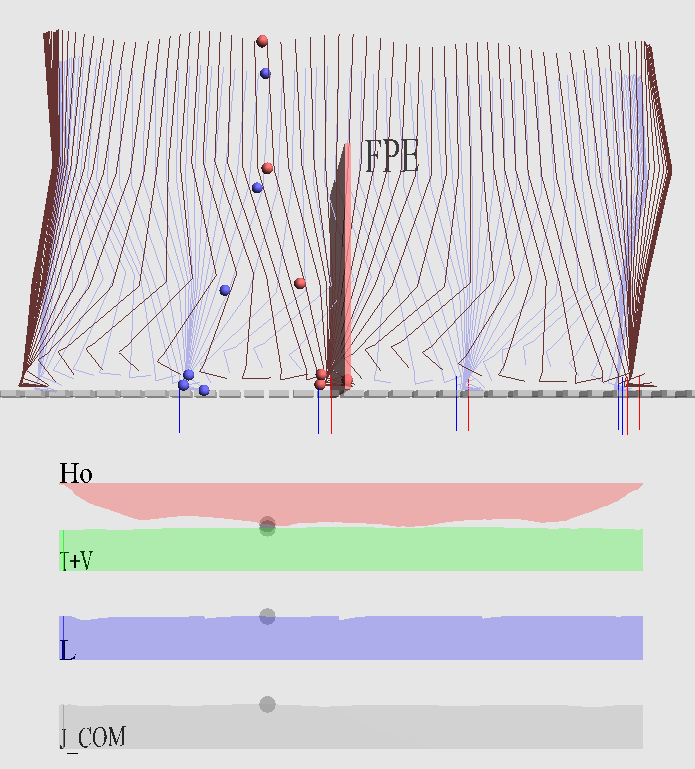
\includegraphics[width = \textwidth, height = 0.5\textheight, keepaspectratio= true]{fig_expData}
\caption{Four integrated data plots are shown in the figure labeled
`Ho', `T+V', `L', and `J\_COM'. These four plots are relevant to the
underlying calculation that governs the location of the `FPE' wall
--- thus saving the viewer from switching between multiple windows. \label{fig_expData}}
\end{figure}

To create a 3D plot the data for the plot must be stored in a text
file and an entry in the *.s4d configuration file must be made so
that Solvere4D renders it properly. The plot data file should have
the following format:

\vspace{1cm}
\begin{center}
\begin{tabular}{c|c|c|c|c|c|c|c|}
\hline Column & 1 & 2 & 3 & 4 & 5 & 6 & 7 \\
\hline & Time & $X_1$ & $Y_1$ & $Z_1$ & $X_2$ & $Y_2$ & $Z_2$\\
\end{tabular}
\end{center}
\vspace{1cm}

Where ($X_1, Y_1, Z_1$) is by default associated with the reference
axis, and ($X_2, Y_2, Z_2$) is the data point. The data marker (the
grey dots in Fig. \ref{fig_expData} will follow the path laid out by
the series of ($X_2, Y_2, Z_2$) points. An example entry in the
*.s4d file to include and render a plot is shown below, and also in
Appendix \ref{app_ex_s4d_Files}.

\vspace{1cm}
\footnotesize
\hlstd{\\
}\hlkey{$<$plot3D$>$}\hlstd{\\
\hlstd{}ankleLeftTorquePLOTY.dat,}\hlkey{$<$w}\hlnum{1\ }\hlkey{R}\hlnum{0.0\ }\hlkey{G}\hlnum{0.0\ }\hlkey{B}\hlnum{0.5\ }\hlkey{T}\hlnum{0.5\ }\hlkey{s}\hlnum{0.075\ }\hlkey{m}\hlnum{1\ }\hlkey{R}\hlnum{1.0\ }\hlkey{G}\hlnum{0.0\ }\hlkey{B}\hlnum{0.0\ }\hlkey{}\hlstr{"Ankle\ Torque"}\hlkey{\ R}\hlnum{0.0\ }\hlkey{G}\hlnum{0.0\ }\hlkey{B}\hlnum{0.0}\hlkey{$>$}\hlstd{\\
\hlstd{ }kneeLeftTorquePLOTY.dat,\ }\hlkey{$<$w}\hlnum{1\ }\hlkey{R}\hlnum{0.0\ }\hlkey{G}\hlnum{0.0\ }\hlkey{B}\hlnum{0.5\ }\hlkey{T}\hlnum{0.5\ }\hlkey{s}\hlnum{0.075\ }\hlkey{m}\hlnum{1\ }\hlkey{R}\hlnum{1.0\ }\hlkey{G}\hlnum{0.0\ }\hlkey{B}\hlnum{0.0\ }\hlkey{}\hlstr{"Knee\ Torque"}\hlkey{\hlstd{\ \ }R}\hlnum{0.0\ }\hlkey{G}\hlnum{0.0\ }\hlkey{B}\hlnum{0.0}\hlkey{$>$}\hlstd{\\
\hlstd{ }hipLeftTorquePLOTY.dat,\hlstd{\ \ }}\hlkey{$<$w}\hlnum{1\ }\hlkey{R}\hlnum{0.0\ }\hlkey{G}\hlnum{0.0\ }\hlkey{B}\hlnum{0.5\ }\hlkey{T}\hlnum{0.5 \ }\hlkey{s\ }\hlnum{0.075\ }\hlkey{m}\hlnum{1\ }\hlkey{R}\hlnum{1.0\ }\hlkey{G}\hlnum{0.0\ }\hlkey{B}\hlnum{0.0\ }\hlkey{}\hlstr{"Hip\ Torque"}\hlkey{\hlstd{\ \ \ }R}\hlnum{0.0\ }\hlkey{G}\hlnum{0.0\ }\hlkey{B}\hlnum{0.0}\hlkey{$>$}\hlstd{\\
}\hlkey{$<$$\backslash$plot3D$>$}
\normalsize
\vspace{1cm}

The plot tag entry is the most elaborate tag in the entire *.s4d
configuration file. The following table will define, element by
element, in the order they appear (from left to right), what each of
the flags in the entries controls:

\vspace{1cm}
\begin{tabular}{l l l}
\hline Flag & Arguments  & Description \\
\hline w & 0 or 1 & Wireframe (0), or solid (1) \\
R G B & & RGB colour the plot is rendered in\\
s & \# $>$ 0 & The scale of the plot label \& marker \\
m & 0 or 1 & Add an animated marker (1) or not (0) \\
R G B & & RGB colour of the marker\\
"Plot Label" & text & The name of the plot, in quotations\\
R G B & & RGB colour of the label\\
\end{tabular}
\vspace{1cm}

If the use of the "R G B" flags to specify colour are unfamiliar to
you please refer to Appendix \ref{app_colour}. An example of both
the plot3D *.dat files and the corresponding entries in the *.s4d
file can be found in both the `Examples/experimental\_data'.

\subsection{$<$stickFigures$>$: Stick Figures Tag}

Static arrays of lines can be printed to the screen using the
$<$stickFigures$>$ tag. This capability can be used to print the
kinematic history of an animation to combine the advantages of a
plots persistent data with the richness of an animation. This
feature is used in `Examples/experimental\_data/fpe\_research.wrl'
and is shown in Fig. \ref{fig_expData} to illustrate the kinematic
history of the person as they jump. This feature was also used to
show the location of foot contact (the blue vertical line) and the
location where foot contact was predicted to occur (shown as a red
vertical line).

To include stick figure drawings in your animation, you must include
a data file that contains the geometry of the stick figures along
with a corresponding entry in the *.s4d configuration file. The data
file should have the following format:

\vspace{1cm}
\begin{center}
\begin{tabular}{c|c|c|c|c|c|c|c|c}
\hline Column & 1 & 2 & 3 & 4 & 5 & 6 & 7 & 8 \ldots \\
\hline & Time & $X_1$ & $Y_1$ & $Z_1$ & $X_2$ & $Y_2$ & $Z_2$  & \ldots\\
\end{tabular}
\end{center}
\vspace{1cm}

Any number of points can be included to draw a single stick figure.
All of the points in one row are interpreted as belonging to a
single stick figure, with subsequent stick figure coordinates being
placed on a new line. The rows within one file must all contain the
same number of coordinates --- if you need to draw another stick
figure that has a different number of points, then you must put that
information in a new file. An example of the *.s4d entry to include
a stick figure is shown below and in Appendix
\ref{app_ex_s4d_Files}.

\vspace{1cm}
\hlstd{\\
}\hlkey{$<$stickFigures$>$}\hlstd{\\
\hlstd{\ \ \ \ }motionL\textunderscore SF.dat,\hlstd{\ \ \ }}\hlkey{$<$R}\hlnum{0.7\ }\hlkey{G}\hlnum{0.7\ }\hlkey{B}\hlnum{0.9}\hlkey{$>$}\hlstd{\\
\hlstd{\ \ \ \ }motionR\textunderscore SF.dat,\hlstd{\ \ \ }}\hlkey{$<$R}\hlnum{0.4\ }\hlkey{G}\hlnum{0.2\ }\hlkey{B}\hlnum{0.2}\hlkey{$>$}\hlstd{\\
\hlstd{\ \ \ \ }FPE\textunderscore SF.dat,\hlstd{\ \ \ \ \ \ \ }}\hlkey{$<$R}\hlnum{1.0\ }\hlkey{G}\hlnum{0.0\ }\hlkey{B}\hlnum{0.0}\hlkey{$>$}\hlstd{\\
\hlstd{\ \ \ \ }HFP\textunderscore SF.dat,\hlstd{\ \ \ \ \ \ }}\hlkey{$<$R}\hlnum{0.0\ }\hlkey{G}\hlnum{0.0\ }\hlkey{B}\hlnum{1.0}\hlkey{$>$}\hlstd{\\
}\hlkey{$<$$\backslash$stickFigures$>$}\hlstd{}\mbox{} \vspace{1cm}

The stick figure lines can be rendered in one colour, dictated by
the values placed after the ``R G B" flags. For more information
refer to Appendix \ref{app_colour}.

\vspace{1cm}
\begin{tabular}{l l l}
\hline Flag & Arguments  & Description \\
R G B & & RGB colour the stick figure lines\\
\end{tabular}
\vspace{1cm}

An example of both the plot3D *.dat files and the corresponding
entries in the *.s4d file can be found in both the
`Examples/experimental\_data'.

\subsection{$<$movingLabels$>$: Moving Labels Tag}

Occasionally it is useful to be able to label different portions of
a particular animation, and to have those labels follow element of
interest. To that end the $<$movingLabels$>$ tag was created. The
label that follows the red wall in the file
`Examples/experimental\_data/fpe\_research.wrl' was created using
this tag.

To apply a moving label to an animation you need to have a data file
that specifies where the label should be as a function of time. As
with every external file used in Solvere4D this file should be tab
delimited and it should have the same number of rows as every other
text file that includes a ``Time" column. The file should have the
following format:

\vspace{1cm}
\begin{center}
\begin{tabular}{c|c|c|c|}
\hline Column & 1 & 2 & 3 \\
\hline  Time & X & Y & Z \\
\end{tabular}
\end{center}
\vspace{1cm}

An entry in the *.s4d configuration file is required to command
Solvere4D to include the label in the animation. An example of this
entry is shown below:

\vspace{1cm}
\hlstd{\\
}\hlkey{$<$movingLabels$>$}\hlstd{\\
\hlstd{\ \ \ \ }FPELabel.dat,\ }\hlkey{$<$}\hlstr{"FPE"}\hlkey{\ s}\hlnum{0.25\ }\hlkey{R}\hlnum{0.10\hlstd{\ \ }}\hlkey{G}\hlnum{0.10\hlstd{\ \ }}\hlkey{B}\hlnum{0.10}\hlkey{$>$}\hlstd{\\
}\hlkey{$<$$\backslash$movingLabels$>$}
\vspace{1cm}

An explanation for each of the flags used in the label tag are shown
below:

\vspace{1cm}
\begin{tabular}{l l l}
\hline Flag & Arguments  & Description \\
\hline "Label Text Here" & Text & The label text \\
s & \# $>$ 0 & The scale of the plot label. \\
& & A "1" will make 1 m tall lettering\\
R G B & & RGB colour the plot is rendered in\\
\end{tabular}
\vspace{1cm}


\newpage
\section{Contributing to Solvere4D}

Solvere4D is free software that is offered under the GNU Public
License or GPL for short. That means that you, the user, have access
to the source code. You may read the code in order to understand how
Solvere4D works and improve it if you like. I have carefully
documented every function and class and named variables in a helpful
manner to make Solvere4D's implementation as understandable as
possible. Solvere4D is written using Java, to make it compatible
with different platforms. Solvere4D functions works in the following
manner, and has different files associated with each function:

\begin{enumerate}
\item Read the *.s4d file and corresponding data files.
\begin{itemize}
\item Solvere4D.java, \emph{readAnimationData} function
\item SolvereUtilities.java, the following functions
\begin{itemize}
\item \emph{parseNumber}
\item \emph{parseRGBT}
\end{itemize}
\item TextParser.java
\end{itemize}

\item Store the information required to build each element in a
class, that functions like a structure. There is a one-to-one
correspondence between *.s4d tags and these storage classes.
\begin{itemize}
\item BodyData.java
\item ForceTorqueData.java
\item Plot3D.java
\item MarkerData.java
\item StickFigure.java
\item Label3D.java
\end{itemize}

\item Alter the data as necessary so that a VRML viewer can display
it.
\begin{itemize}
\item SolvereUtilities.java, with the following functions:
\begin{itemize}
\item \emph{convertToQuat}
\item \emph{getAxisAngle}
\item \emph{getColourMapping}
\item \emph{getTriangularArray}
\end{itemize}
\end{itemize}

\item Write the data to a VRML file. This is done by reading in a
VRML file for each tag element and replacing data in the default
file with data specific to the users animation.
\begin{itemize}
\item Solvere4D.java, \emph{writeAnimationData} function
\item SolvereUtilities.java, with the following functions:
\begin{itemize}
\item \emph{appendColourTag}
\item \emph{appendHeader}
\item \emph{appendMovingLabel}
\item \emph{appendOrientationTag}
\item \emph{appendPlot}
\item \emph{appendRouteColour}
\item \emph{appendRouteRotation}
\item \emph{appendRouteTranslation}
\item \emph{appendScaleTag}
\item \emph{appendStaticMarker}
\item \emph{appendStickFigure}
\item \emph{appendTimeControls}
\item \emph{appendTranslationTag}
\item \emph{getTextFile}
\item \emph{mergStrings}
\item \emph{replaceTags}
\end{itemize}
\item All of the `lib\_' files in `build/classes/WRL\_SYNTAX'
\end{itemize}
\end{enumerate}

Every function and every file is commented. If you're interested in
adding a function to Solvere4D I suggest you go and download Sun's
free Java developer environment and start stepping through the code
to get a better feel for how it works. If you'd like to contribute
but do not know what to contribute, here are a list of things I
would like to add to Solvere4D, but have not yet:

\begin{enumerate}
\item Update Solvere4D to export X3D. This would come in 2 parts:

\begin{enumerate}
\item Create a series of `lib\_' files just as in
`build/classes/WRL\_SYNTAX', but for *.x3d files and in a folder
called `build/classes/X3D\_SYNTAX'
\item Update Solvere4D to output an X3D file - this involves
upgrades to the `readAnimationFile' function in Solvere4D.java and
the `append \ldots' functions in `SolvereUtilities.java'.
\end{enumerate}

\item Add the capability to display deformable geometry, and
eventually muscle.

\end{enumerate}





\appendix
\newpage
\section{Colour in Solvere4D}
\label{app_colour} Many tags in Solvere4D allow you to set the
colour of a particular element. In Solvere4D it is expected that you
enter the colour using its Red-Green-Blue (RGB) colour space value.
This involves entering 3 numbers that correspond to the right mix of
red, green and blue in order to create the colour you are interested
in. The table below contains some basic colour entries that you can
use for your convenience:

\vspace{1cm}

\begin{tabular}{l l}
\hline RGB Text & Common Name \\
\hline R0.0 G0.0 B0.0 & Black \\
R0.0 G0.0 B1.0 & Blue \\
R0.0 G1.0 B0.0 & Green \\
R0.0 G1.0 B1.0 & Cyan \\
R1.0 G0.0 B0.0 & Red \\
R1.0 G0.0 B1.0 & Magenta \\
R1.0 G1.0 B0.0 & Yellow \\
R1.0 G1.0 B1.0 & White \\
&  \\
R0.1 G0.1 B0.1 & Dark Gray\\
R0.5 G0.5 B0.5 & Medium Gray\\
R0.9 G0.9 B0.9 & Light Gray\\
\end{tabular}

\vspace{1cm}

Further adjusting these values will allow you to create what ever
hue you want. For example, if you wanted a Sienna Brown you would
use red with some green and blue: "R0.63 G0.32 B0.18". The internet
is a great resource for finding RGB colour values, though the amount
of each colour is usually specified as an integer from 0-255, that
is as an 8 bit number. Thus Sienna Brown would be 160 82 45. To
convert the values to 0-1 decimal values, simply divide each entry
by 255. An excellent reference can be found in the document titled
``Loreti\_rgb.pdf" that is in Solvere4D's ``Manual" folder.

\section{Example s4d Configuration Files}
\label{app_ex_s4d_Files} The following shows: airWalkHat.sd4

\begin{landscape}
\footnotesize \noindent \ttfamily
\hlstd{}\hlkey{$<$timeScaling$>$}\hlstd{,\hlstd{\ \ \ \ }}\hlnum{1.0\\
}\hlstd{}\hlkey{$<$downSampling$>$}\hlstd{,\hlstd{\ \ \ \ }}\hlnum{2\\
}\hlstd{}\hlkey{$<$backgroundColour$>$}\hlstd{,\hlstd{\ \ }}\hlkey{$<$R}\hlnum{0.90\ }\hlkey{G}\hlnum{0.90\ }\hlkey{B}\hlnum{0.90}\hlkey{$>$}\hlstd{\\
}\hlkey{$<$lightDirection$>$}\hlstd{,\ }\hlkey{$<$X}\hlnum{-0.5\ }\hlkey{Y}\hlnum{-0.5\ }\hlkey{Z}\hlnum{-1}\hlkey{$>$}\hlstd{\\
}\hlkey{$<$headlight$>$}\hlstd{,\ }\hlnum{0\\
}\hlstd{}\hlkey{$<$bodyGEO$>$}\hlstd{,}\hlkey{$<$bodiesMOV$>$}\hlstd{\\
\hlstd{\ \ \ \ }hat.wrl,\hlstd{\ \ \ \ \ }HatPosOrien.dat\\
\hlstd{\ \ \ \ }thighL.wrl,\hlstd{\ \ \ \ }HipLeftJointPosOrien.dat\\
\hlstd{\ \ \ \ }shinL.wrl,\hlstd{\ \ \ \ }KneeLeftJointPosOrien.dat\\
\hlstd{\ \ \ \ }footL.wrl,\hlstd{\ \ \ \ }AnkleLeftJointPosOrien.dat\\
\hlstd{\ \ \ \ }thigh.wrl,\hlstd{\ \ \ \ }HipRightJointPosOrien.dat\\
\hlstd{\ \ \ \ }shin.wrl,\hlstd{\ \ \ \ }KneeRightJointPosOrien.dat\\
\hlstd{\ \ \ \ }foot.wrl,\hlstd{\ \ \ \ }AnkleRightJointPosOrien.dat\\
\hlstd{\ \ \ \ }contact.wrl,\hlstd{\ \ \ \ }heelRightPosOrien.dat\\
\hlstd{\ \ \ \ }contact.wrl,\hlstd{\ \ \ \ }heelLeftPosOrien.dat\\
\hlstd{\ \ \ \ }contact.wrl,\hlstd{\ \ \ \ }toeRightPosOrien.dat\\
\hlstd{\ \ \ \ }contact.wrl,\hlstd{\ \ \ \ }toeLeftPosOrien.dat\\
}\hlkey{$<$$\backslash$bodyGEO$>$}\hlstd{,}\hlkey{$<$$\backslash$bodiesMOV$>$}\hlstd{\\
}\hlkey{$<$forceTorque$>$}\hlstd{,}\hlkey{$<$genForceTorquePlots$>$}\hlstd{\ normF=}\hlnum{1000.0\ }\hlstd{normT=}\hlnum{500.0\ }\hlstd{normD=}\hlnum{1.0\\
\hlstd{\ \ \ \ }}\hlstd{toeRightForces.dat,\hlstd{\ \ }}\hlkey{$<$f}\hlnum{0\ }\hlkey{w}\hlnum{0\ }\hlkey{c}\hlnum{0\ }\hlkey{R}\hlnum{0.0\ }\hlkey{G}\hlnum{0.0\ }\hlkey{B}\hlnum{0.5\ }\hlkey{T}\hlnum{0.5}\hlkey{$>$}\hlstd{\ }\hlkey{$<$t}\hlnum{0\ }\hlkey{w}\hlnum{1\ }\hlkey{c}\hlnum{1\ }\hlkey{R}\hlnum{1.0\ \ }\hlkey{G}\hlnum{0.5\ \ }\hlkey{B}\hlnum{0.0\ \ \ }\hlkey{T}\hlnum{0.5}\hlkey{$>$}\hlstd{\\
\hlstd{\ \ \ \ }heelRightForces.dat,\ }\hlkey{$<$f}\hlnum{0\ }\hlkey{w}\hlnum{0\ }\hlkey{c}\hlnum{0\ }\hlkey{R}\hlnum{0.0\ }\hlkey{G}\hlnum{0.0\ }\hlkey{B}\hlnum{1.0\ }\hlkey{T}\hlnum{0.5}\hlkey{$>$}\hlstd{\ }\hlkey{$<$t}\hlnum{0\ }\hlkey{w}\hlnum{1\ }\hlkey{c}\hlnum{1\ }\hlkey{R}\hlnum{0.0\ \ }\hlkey{G}\hlnum{0.5\ \ }\hlkey{B\ }\hlnum{1.0\ \ \ }\hlkey{T}\hlnum{0.5}\hlkey{$>$}\hlstd{\\
\hlstd{\ \ \ \ }leftGRF.dat,\hlstd{\ \ \ \ \ \ \ \ \ }}\hlkey{$<$f}\hlnum{0\ }\hlkey{w}\hlnum{0\ }\hlkey{c}\hlnum{0\ }\hlkey{R}\hlnum{1.0\ }\hlkey{G}\hlnum{0.2\ }\hlkey{B}\hlnum{0.2\ }\hlkey{T}\hlnum{0.5}\hlkey{$>$}\hlstd{\ }\hlkey{$<$t}\hlnum{0\ }\hlkey{w}\hlnum{1\ }\hlkey{c}\hlnum{1\ }\hlkey{R}\hlnum{1.5\ \ }\hlkey{G}\hlnum{1.0\ \ }\hlkey{B}\hlnum{0.0\ \ \  }\hlkey{T}\hlnum{0.5}\hlkey{$>$}\hlstd{\\
\hlstd{\ \ \ \ }hipLeftTorque.dat,\hlstd{\ \ \ }}\hlkey{$<$f}\hlnum{0\ }\hlkey{w}\hlnum{1\ }\hlkey{c}\hlnum{1\ }\hlkey{R}\hlnum{0.0\ }\hlkey{G}\hlnum{1.0\ }\hlkey{B}\hlnum{1.0\ }\hlkey{T}\hlnum{0.5}\hlkey{$>$}\hlstd{\ }\hlkey{$<$t}\hlnum{0\ }\hlkey{w}\hlnum{1\ }\hlkey{c}\hlnum{1\ }\hlkey{R}\hlnum{0.33\ }\hlkey{G}\hlnum{0.0\hlstd{\ \ }}\hlkey{B}\hlnum{0.33\ \ }\hlkey{T}\hlnum{0.5}\hlkey{$>$}\hlstd{\\
\hlstd{\ \ \ \ }hipRightTorque.dat,\hlstd{\ \  }}\hlkey{$<$f}\hlnum{0\ }\hlkey{w}\hlnum{1\ }\hlkey{c}\hlnum{1\ }\hlkey{R}\hlnum{0.5\ }\hlkey{G}\hlnum{0.5\ }\hlkey{B}\hlnum{1.0\ }\hlkey{T}\hlnum{0.5}\hlkey{$>$}\hlstd{\ }\hlkey{$<$t}\hlnum{0\ }\hlkey{w}\hlnum{1\ }\hlkey{c}\hlnum{1\ }\hlkey{R}\hlnum{0.33\ }\hlkey{G}\hlnum{0.33\ }\hlkey{B}\hlnum{0.0\ \ \ }\hlkey{T}\hlnum{0.5}\hlkey{$>$}\hlstd{\\
\hlstd{\ \ \ \ }kneeLeftTorque.dat,\hlstd{\ \  }}\hlkey{$<$f}\hlnum{0\ }\hlkey{w}\hlnum{1\ }\hlkey{c}\hlnum{1\ }\hlkey{R}\hlnum{0.5\ }\hlkey{G}\hlnum{0.5\ }\hlkey{B}\hlnum{1.0\ }\hlkey{T}\hlnum{0.5}\hlkey{$>$}\hlstd{\ }\hlkey{$<$t}\hlnum{0\ }\hlkey{w}\hlnum{1\ }\hlkey{c}\hlnum{1\ }\hlkey{R}\hlnum{0.67\ }\hlkey{G}\hlnum{0.0\hlstd{\ \ }}\hlkey{B}\hlnum{0.67\ \  }\hlkey{T}\hlnum{0.5}\hlkey{$>$}\hlstd{\\
\hlstd{\ \ \ \ }kneeRightTorque.dat,\ }\hlkey{$<$f}\hlnum{0\ }\hlkey{w}\hlnum{1\ }\hlkey{c}\hlnum{1\ }\hlkey{R}\hlnum{0.5\ }\hlkey{G}\hlnum{0.5\ }\hlkey{B}\hlnum{1.0\ }\hlkey{T}\hlnum{0.5}\hlkey{$>$}\hlstd{\ }\hlkey{$<$t}\hlnum{0\ }\hlkey{w}\hlnum{1\ }\hlkey{c}\hlnum{1\ }\hlkey{R}\hlnum{0.67\ }\hlkey{G}\hlnum{0.67\ }\hlkey{B}\hlnum{0.0\ \ \ }\hlkey{T}\hlnum{0.5}\hlkey{$>$}\hlstd{\\
\hlstd{\ \ \ \ }ankleLeftTorque.dat,\ }\hlkey{$<$f}\hlnum{0\ }\hlkey{w}\hlnum{1\ }\hlkey{c}\hlnum{1\ }\hlkey{R}\hlnum{0.5\ }\hlkey{G}\hlnum{0.5\ }\hlkey{B}\hlnum{1.0\ }\hlkey{T}\hlnum{0.5}\hlkey{$>$}\hlstd{\ }\hlkey{$<$t}\hlnum{0\ }\hlkey{w}\hlnum{0\ }\hlkey{c}\hlnum{1\ }\hlkey{R}\hlnum{1.0\hlstd{\ \ }}\hlkey{G}\hlnum{0.0\hlstd{\ \ }}\hlkey{B}\hlnum{1.0\ \ \ }\hlkey{T}\hlnum{0.25}\hlkey{$>$}\hlstd{\\
\hlstd{\ \ \ \ }ankleRightTorque.dat,}\hlkey{$<$f}\hlnum{0\ }\hlkey{w}\hlnum{1\ }\hlkey{c}\hlnum{1\ }\hlkey{R}\hlnum{0.5\ }\hlkey{G}\hlnum{0.5\ }\hlkey{B}\hlnum{1.0\ }\hlkey{T}\hlnum{0.5}\hlkey{$>$}\hlstd{\ }\hlkey{$<$t}\hlnum{0\ }\hlkey{w}\hlnum{1\ }\hlkey{c}\hlnum{1\ }\hlkey{R}\hlnum{1.0\hlstd{\ \ }}\hlkey{G}\hlnum{1.0\hlstd{\ \ }}\hlkey{B}\hlnum{0.0\ \ \ }\hlkey{T}\hlnum{0.5}\hlkey{$>$}\hlstd{\\
}\hlkey{$<$$\backslash$forceTorque$>$}\hlstd{,}\hlkey{$<$$\backslash$genForcePlots$>$}\hlstd{,}\hlkey{$<$$\backslash$genTorquePlots$>$}\hlstd{\\
}\hlkey{$<$camera$>$}\hlstd{\\
\hlstd{\ \ \ \ }cameraPosOrien.dat\\
}\hlkey{$<$$\backslash$camera$>$}\hlstd{\\
}\hlkey{$<$markers$>$}\hlstd{\\
\hlstd{\ \ \ \ }gridMarkers.txt,\hlstd{\ \ }}\hlkey{$<$sphere\ r}\hlnum{0.02\hlstd{\ \ \ \ \ \ \ \ \ \ \ \ \ \ \ \ \ \ \ \ \ \ }}\hlkey{R}\hlnum{0.6\ }\hlkey{G}\hlnum{0.6\ }\hlkey{B}\hlnum{0.9\ }\hlkey{T}\hlnum{0.0}\hlkey{$>$}\hlstd{\\
\hlstd{\ \ \ \ }floorMarkers.txt,\hlstd{\ \ }}\hlkey{$<$box\hlstd{\ \ \ \ }x}\hlnum{0.05\ }\hlkey{y}\hlnum{0.01\ }\hlkey{z}\hlnum{0.2\hlstd{\ \ \ \ \ }}\hlkey{R}\hlnum{0.6\ }\hlkey{G}\hlnum{0.6\ }\hlkey{B}\hlnum{0.8\ }\hlkey{T}\hlnum{0.0}\hlkey{$>$}\hlstd{\\
\hlstd{\ \ \ \ }xyGridMarkers.txt,\ }\hlkey{$<$sphere\ r}\hlnum{0.01\hlstd{\ \ \ \ \ \ \ \ \ \ \ \ \ \ \ \ \ \ \ \ \ }}\hlkey{R}\hlnum{0.0\ }\hlkey{G}\hlnum{0.0\ }\hlkey{B}\hlnum{0.8\ }\hlkey{T}\hlnum{0.0}\hlkey{$>$}\hlstd{\\
}\hlkey{$<$$\backslash$markers$>$}\hlstd{\\
\#}\hlkey{$<$plot3D$>$}\hlstd{\\
\hlstd{\ \ \ \ }ankleLeftTorquePLOTY.dat,}\hlkey{$<$w}\hlnum{1\ }\hlkey{R}\hlnum{0.0\ }\hlkey{G}\hlnum{0.0\ }\hlkey{B}\hlnum{0.5\ }\hlkey{T}\hlnum{0.5\hlstd{\ \ }}\hlkey{s}\hlnum{0.075\ }\hlkey{m}\hlnum{1\ }\hlkey{R}\hlnum{1.0\ }\hlkey{G}\hlnum{0.0\ }\hlkey{B}\hlnum{0.0\ }\hlkey{}\hlstr{"Ankle\ Torque"}\hlkey{\ R}\hlnum{0.0\ }\hlkey{G}\hlnum{0.0\ }\hlkey{B}\hlnum{0.0}\hlkey{$>$}\hlstd{\\
\hlstd{\ \ \ \ }kneeLeftTorquePLOTY.dat,\ }\hlkey{$<$w}\hlnum{1\ }\hlkey{R}\hlnum{0.0\ }\hlkey{G}\hlnum{0.0\ }\hlkey{B}\hlnum{0.5\ }\hlkey{T}\hlnum{0.5\hlstd{\ \ }}\hlkey{s}\hlnum{0.075\ }\hlkey{m}\hlnum{1\ }\hlkey{R}\hlnum{1.0\ }\hlkey{G}\hlnum{0.0\ }\hlkey{B}\hlnum{0.0\ }\hlkey{}\hlstr{"Knee\ Torque"}\hlkey{\hlstd{\ \ }R}\hlnum{0.0\ }\hlkey{G}\hlnum{0.0\ }\hlkey{B}\hlnum{0.0}\hlkey{$>$}\hlstd{\\
\hlstd{\ \ \ \ }hipLeftTorquePLOTY.dat,\hlstd{\ \ }}\hlkey{$<$w}\hlnum{1\ }\hlkey{R}\hlnum{0.0\ }\hlkey{G}\hlnum{0.0\ }\hlkey{B}\hlnum{0.5\ }\hlkey{T}\hlnum{0.5\hlstd{\ \ }}\hlkey{s\ }\hlnum{0.075\ }\hlkey{m}\hlnum{1\ }\hlkey{R}\hlnum{1.0\ }\hlkey{G}\hlnum{0.0\ }\hlkey{B}\hlnum{0.0\ }\hlkey{}\hlstr{"Hip\ Torque"}\hlkey{\hlstd{\ \ \ }R}\hlnum{0.0\ }\hlkey{G}\hlnum{0.0\ }\hlkey{B}\hlnum{0.0}\hlkey{$>$}\hlstd{\\
}\hlkey{$<$$\backslash$plot3D$>$}\hlstd{\\
}\hlkey{$<$stickFigures$>$}\hlstd{\\
\hlstd{\ \ \ \ }stickfigure.dat,\ }\hlkey{$<$R}\hlnum{0\ }\hlkey{G}\hlnum{0\ }\hlkey{B}\hlnum{0\ }\hlkey{$>$}\hlstd{\\
}\hlkey{$<$$\backslash$stickFigures$>$}\hlstd{\\
\#}\hlkey{$<$movingLabels$>$}\hlstd{\\
\hlstd{\ \ \ \ }larryLabel.dat,\ }\hlkey{$<$}\hlstr{"Larry"}\hlkey{\ s}\hlnum{0.5\ }\hlkey{R}\hlnum{0.0\hlstd{\ \ }}\hlkey{G}\hlnum{0.0\hlstd{\ \ }}\hlkey{B}\hlnum{1.0}\hlkey{$>$}\hlstd{\\
}\hlkey{$<$$\backslash$movingLabels$>$}\hlstd{\mbox{}\\
\\
Anything\ that\ is\ not\ betwetween\ a\ recognized\ tag\ such\ as\ those\ above,\\
int\ the\ angled\ brackets,\ is\ treated\ as\ a\ comment.\mbox{}\\
\\
If\ the\ tags\ in\ the\ square\ brackets\ have\ any\ other\ character\ (such\ as\ the\\
}\hlstr{"\#"}\hlstd{\ in\ front\ of\ the\ moving\ Label)\ then\ the\ whole\ block\ is\ ignored.\ At\\
the\ moment\ there\ is\ no\ way\ to\ comment\ out\ a\ single\ entry\ for\ a\ given\\
tag,\ you\ just\ have\ to\ move\ it\ outside\ from\ its\ tagged\ region.}\mbox{}\\
\mbox{}\\
\normalfont
\end{landscape}

\newpage
fpe\_research.s4d

\begin{landscape}
\noindent \ttfamily \footnotesize
\hlstd{}\hlkey{$<$timeScaling$>$}\hlstd{,\hlstd{\ \ \ \ }}\hlnum{1.0\\
}\hlstd{}\hlkey{$<$downSampling$>$}\hlstd{,\hlstd{\ \ \ \ }}\hlnum{4\\
}\hlstd{}\hlkey{$<$lightDirection$>$}\hlstd{,\hlstd{\ \ }}\hlkey{$<$X}\hlnum{-0.5\ }\hlkey{Y}\hlnum{-0.5\ }\hlkey{Z}\hlnum{-1}\hlkey{$>$}\hlstd{\\
}\hlkey{$<$headlight$>$}\hlstd{,\ }\hlnum{0\\
}\hlstd{}\hlkey{$<$backgroundColour$>$}\hlstd{,\ }\hlkey{$<$R}\hlnum{0.9\ }\hlkey{G}\hlnum{0.9\ }\hlkey{B}\hlnum{0.9}\hlkey{$>$}\hlstd{\\
}\hlkey{$<$bodyGEO$>$}\hlstd{,}\hlkey{$<$bodiesMOV$>$}\hlstd{\\
\hlstd{\ \ \ \ }redsphere.wrl,\hlstd{\ \ \ \ }M1.dat\\
\hlstd{\ \ \ \ }redsphere.wrl,\hlstd{\ \ \ \ }M2.dat\\
\hlstd{\ \ \ \ }redsphere.wrl,\hlstd{\ \ \ \ }M3.dat\\
\hlstd{\ \ \ \ }redsphere.wrl,\hlstd{\ \ \ \ }M4.dat\\
\hlstd{\ \ \ \ }redsphere.wrl,\hlstd{\ \ \ \ }M5.dat\\
\hlstd{\ \ \ \ }redsphere.wrl,\hlstd{\ \ \ \ }M6.dat\\
\hlstd{\ \ \ \ }bluesphere.wrl,\hlstd{\ \ \ \ }M7.dat\\
\hlstd{\ \ \ \ }bluesphere.wrl,\hlstd{\ \ \ \ }M8.dat\\
\hlstd{\ \ \ \ }bluesphere.wrl,\hlstd{\ \ \ \ }M9.dat\\
\hlstd{\ \ \ \ }bluesphere.wrl,\hlstd{\ \ \ \ }M10.dat\\
\hlstd{\ \ \ \ }bluesphere.wrl,\hlstd{\ \ \ \ }M11.dat\\
\hlstd{\ \ \ \ }bluesphere.wrl,\hlstd{\ \ \ \ }M12.dat\\
\hlstd{\ \ \ \ }redplane.wrl,\hlstd{\ \ \ \ }FPEX.dat\\
}\hlkey{$<$$\backslash$bodyGEO$>$}\hlstd{,}\hlkey{$<$$\backslash$bodiesMOV$>$}\hlstd{\\
}\hlkey{$<$camera$>$}\hlstd{\\
\hlstd{\ \ \ \ }cameraPosOrien.dat\\
}\hlkey{$<$$\backslash$camera$>$}\hlstd{\\
}\hlkey{$<$plot3D$>$}\hlstd{\\
\hlstd{\ \ \ \ }Ho.dat,\hlstd{\ \ \ \ \ \ \ \ }}\hlkey{$<$w}\hlnum{0\ }\hlkey{R}\hlnum{0.5\hlstd{\ \ }}\hlkey{G}\hlnum{0.0\hlstd{\ \ }}\hlkey{B}\hlnum{0.0\hlstd{\ \ }}\hlkey{T}\hlnum{0.75\hlstd{\ \ }}\hlkey{s}\hlnum{0.15\ }\hlkey{m}\hlnum{1\ }\hlkey{R}\hlnum{0.0\ }\hlkey{G}\hlnum{0.0\ }\hlkey{B}\hlnum{0.0\ }\hlkey{}\hlstr{"Ho"}\hlkey{\hlstd{\ \ \ \ \ }R}\hlnum{0.0\hlstd{\ \ }}\hlkey{G}\hlnum{0.0\hlstd{\ \ }}\hlkey{B}\hlnum{0.0}\hlkey{$>$}\hlstd{\\
\hlstd{\ \ \ \ }TpV.dat,\hlstd{\ \ \ \ \ \ \ }}\hlkey{$<$w}\hlnum{0\ }\hlkey{R}\hlnum{0.0\hlstd{\ \ }}\hlkey{G}\hlnum{0.5\hlstd{\ \ }}\hlkey{B}\hlnum{0.0\hlstd{\ \ }}\hlkey{T}\hlnum{0.75\hlstd{\ \ }}\hlkey{s}\hlnum{0.15\ }\hlkey{m}\hlnum{1\ }\hlkey{R}\hlnum{0.0\ }\hlkey{G}\hlnum{0.0\ }\hlkey{B}\hlnum{0.0\ }\hlkey{}\hlstr{"T+V"}\hlkey{\hlstd{\ \ \ }R}\hlnum{0.0\hlstd{\ \ }}\hlkey{G}\hlnum{0.0\hlstd{\ \ }}\hlkey{B}\hlnum{0.0}\hlkey{$>$}\hlstd{\\
\hlstd{\ \ \ \ }L.dat,\hlstd{\ \ \ \ \ \ \ \ \ }}\hlkey{$<$w}\hlnum{0\ }\hlkey{R}\hlnum{0.0\hlstd{\ \ }}\hlkey{G}\hlnum{0.0\hlstd{\ \ }}\hlkey{B}\hlnum{0.5\hlstd{\ \ }}\hlkey{T}\hlnum{0.75\hlstd{\ \ }}\hlkey{s}\hlnum{0.15\ }\hlkey{m}\hlnum{1\ }\hlkey{R}\hlnum{0.0\ }\hlkey{G}\hlnum{0.0\ }\hlkey{B}\hlnum{0.0\ }\hlkey{}\hlstr{"L"}\hlkey{\hlstd{\ \ \ \ \ \ \ }R}\hlnum{0.0\hlstd{\ \ }}\hlkey{G}\hlnum{0.0\hlstd{\ \ }}\hlkey{B}\hlnum{0.0}\hlkey{$>$}\hlstd{\\
\hlstd{\ \ \ \ }JCOM.dat,\hlstd{\ \ \ \ \ \ }}\hlkey{$<$w}\hlnum{0\ }\hlkey{R}\hlnum{0.25\ }\hlkey{G}\hlnum{0.25\ }\hlkey{B}\hlnum{0.25\ }\hlkey{T}\hlnum{0.75\hlstd{\ \ }}\hlkey{s}\hlnum{0.15\ }\hlkey{m}\hlnum{1\ }\hlkey{R}\hlnum{0.0\ }\hlkey{G}\hlnum{0.0\ }\hlkey{B}\hlnum{0.0\ }\hlkey{}\hlstr{"J\textunderscore COM"}\hlkey{\ R}\hlnum{0.0\hlstd{\ \ }}\hlkey{G}\hlnum{0.0\hlstd{\ \ }}\hlkey{B}\hlnum{0.0}\hlkey{$>$}\hlstd{\\
}\hlkey{$<$$\backslash$plot3D$>$}\hlstd{\\
}\hlkey{$<$movingLabels$>$}\hlstd{\\
\hlstd{\ \ \ \ }FPELabel.dat,\ }\hlkey{$<$}\hlstr{"FPE"}\hlkey{\ s}\hlnum{0.25\ }\hlkey{R}\hlnum{0.10\hlstd{\ \ }}\hlkey{G}\hlnum{0.10\hlstd{\ \ }}\hlkey{B}\hlnum{0.10}\hlkey{$>$}\hlstd{\\
}\hlkey{$<$$\backslash$movingLabels$>$}\hlstd{\\
}\hlkey{$<$markers$>$}\hlstd{\\
\hlstd{\ \ \ \ }floorMarkers.txt,\ }\hlkey{$<$box\ x}\hlnum{0.09\ }\hlkey{y}\hlnum{0.03\ }\hlkey{z}\hlnum{0.2\ }\hlkey{R}\hlnum{0.6\ }\hlkey{G}\hlnum{0.6\ }\hlkey{B}\hlnum{0.6\ }\hlkey{T}\hlnum{0.50}\hlkey{$>$}\hlstd{\\
}\hlkey{$<$$\backslash$markers$>$}\hlstd{\\
}\hlkey{$<$stickFigures$>$}\hlstd{\\
\hlstd{\ \ \ \ }motionL\textunderscore SF.dat,\hlstd{\ \ \ }}\hlkey{$<$R}\hlnum{0.7\ }\hlkey{G}\hlnum{0.7\ }\hlkey{B}\hlnum{0.9}\hlkey{$>$}\hlstd{\\
\hlstd{\ \ \ \ }motionR\textunderscore SF.dat,\hlstd{\ \ \ }}\hlkey{$<$R}\hlnum{0.4\ }\hlkey{G}\hlnum{0.2\ }\hlkey{B}\hlnum{0.2}\hlkey{$>$}\hlstd{\\
\hlstd{\ \ \ \ }FPE\textunderscore SF.dat,\hlstd{\ \ \ \ \ \ \ }}\hlkey{$<$R}\hlnum{1.0\ }\hlkey{G}\hlnum{0.0\ }\hlkey{B}\hlnum{0.0}\hlkey{$>$}\hlstd{\\
\hlstd{\ \ \ \ }HFP\textunderscore SF.dat,\hlstd{\ \ \ \ \ \ }}\hlkey{$<$R}\hlnum{0.0\ }\hlkey{G}\hlnum{0.0\ }\hlkey{B}\hlnum{1.0}\hlkey{$>$}\hlstd{\\
}\hlkey{$<$$\backslash$stickFigures$>$}\hlstd{}\mbox{}\\
\mbox{}\\
\normalfont
\end{landscape}

\section{Generating Animations using Solvere4D From Matlab}

\label{app_matlab}

Although Solvere4D cannot be called directly from Matlab, a *.bat
file that runs Solvere4D can be called from Matlab. Matlab can be
used to write and run a *.bat file (which is just a text file with
an extension of *.bat) that will run Solvere4D. While the data files
may be new for every animation you create, you might have a number
of static files (*.wrl geometry files, marker location files, the
*.s4d configuration file) that you need in order to create your
animation file.



\definecolor{bgcolor}{rgb}{1,1,1}
\pagecolor{bgcolor} \noindent \ttfamily
\hlstd{}\hlcom{\%\%\\
}\hlstd{}\hlcom{\%\ Write\ the\ VRML\ data\ files\\
}\hlstd{}\hlcom{\%\%\mbox{}\\
}\hlstd{\\
}\hlkey{if\ }\hlstd{flag\textunderscore genVRMLFiles\ ==\ }\hlnum{1\mbox{}\\
\\
\ }\hlstd{}\hlcom{\%\%\%\%\%\%\%\%\%\%\%\%\%\%\%\%\%\%\%\%\%\%\%\%\%\%\%\%\%\%\%\%\%\%\%\%\%\%\%\%\%\%\%\%\%\%\%\%\%\%\\
}\hlstd{\ }\hlcom{\%\\
}\hlstd{\ }\hlcom{\%\ 1.\ Copy\ over\ the\ files\ in\ the\ support\ directory.\\
}\hlstd{\ }\hlcom{\%\ \ \ This\ includes\ all\ files\ EXCEPT\ the\ *.dat\ files \\
}\hlstd{\ }\hlcom{\%\\
}\hlstd{\ }\hlcom{\%\%\%\%\%\%\%\%\%\%\%\%\%\%\%\%\%\%\%\%\%\%\%\%\%\%\%\%\%\%\%\%\%\%\%\%\%\%\%\%\%\%\%\%\%\%\%\%\%\%\mbox{}\\
}\hlstd{\mbox{}\\
\\
\hlstd{\ \ \ \ }}\hltyp{tempDir\ }\hlstd{=\ }\hlkey{pwd}\hlstd{;\mbox{}\\
\\
\hlstd{\ \ \ \ }aniDir\ =\ ['C:$\backslash$mjhmilla\textunderscore TEMP$\backslash$FPE$\backslash$Animation'];\\
\hlstd{\ \ \ \ }}\hlkey{cd}\hlstd{(aniDir);\\
\hlstd{\ \ \ \ }supDir\ =\ [aniDir,'$\backslash$suppfiles'];\mbox{}\\
\\
\hlstd{\ \ \ \ }subDir\ =\ ['S',}\hltyp{num2str}\hlstd{(i)];\\
\hlstd{\ \ \ \ }expDir\ =\ expName;\\
\hlstd{\ \ \ \ }trialDir\ =\ ['T',}\hltyp{num2str}\hlstd{(k)];\mbox{}\\
\\
\hlstd{\ \ \ \ }}\hlcom{\%\%\\
}\hlstd{\hlstd{\ \ \ \ }}\hlcom{\%Get\ into\ the\ proper\ directory\\
}\hlstd{\hlstd{\ \ \ \ }}\hlcom{\%\%\mbox{}\\
}\hlstd{\\
\hlstd{\ \ \ \ }}\hlkey{if\ }\hlstd{isdir(subDir)\\
\hlstd{\ \ \ \ \ \ \ \ }}\hlkey{cd}\hlstd{(subDir);\\
\hlstd{\ \ \ \ }}\hlkey{else\\
\hlstd{\ \ \ \ \ \ \ \ }}\hlstd{mkdir(subDir);\\
\hlstd{\ \ \ \ \ \ \ \ }}\hlkey{cd}\hlstd{(subDir);\\
\hlstd{\ \ \ \ }}\hlkey{end\mbox{}\\
\\
\hlstd{\ \ \ \ }if\ }\hlstd{isdir(expDir)\\
\hlstd{\ \ \ \ \ \ \ \ }}\hlkey{cd}\hlstd{(expDir);\\
\hlstd{\ \ \ \ }}\hlkey{else\\
\hlstd{\ \ \ \ \ \ \ \ }}\hlstd{mkdir(expDir);\\
\hlstd{\ \ \ \ \ \ \ \ }}\hlkey{cd}\hlstd{(expDir);\\
\hlstd{\ \ \ \ }}\hlkey{end\mbox{}\\
\\
\hlstd{\ \ \ \ }if\ }\hlstd{isdir(trialDir)\\
\hlstd{\ \ \ \ \ \ \ \ }}\hlkey{cd}\hlstd{(trialDir);\\
\hlstd{\ \ \ \ }}\hlkey{else\\
\hlstd{\ \ \ \ \ \ \ \ }}\hlstd{mkdir(trialDir);\\
\hlstd{\ \ \ \ \ \ \ \ }}\hlkey{cd}\hlstd{(trialDir);\\
\hlstd{\ \ \ \ }}\hlkey{end\mbox{}\\
\\
\hlstd{\ \ \ \ }}\hlstd{fileDir\ =\ }\hlkey{pwd}\hlstd{;\mbox{}\\
\\
\ }\hlcom{\%Now\ we\ are\ in\ the\ directory\ we\ would\ like\ to\\
}\hlstd{\ }\hlcom{\%have\ the\ support\ files\ in.\ Time\ to\ get\ DOS\ to\\
}\hlstd{\ }\hlcom{\%copy\ them\ over\ for\ us\mbox{}\\
}\hlstd{\\
\hlstd{\ \ \ \ }}\hlkey{dos}\hlstd{(['xcopy\ ',supDir,\ '\ /e\ /Y']);\mbox{}\\
\\
}\hlcom{\%\%\%\%\%\%\%\%\%\%\%\%\%\%\%\%\%\%\%\%\%\%\%\%\%\%\%\%\%\%\%\%\%\%\%\%\%\%\%\%\%\%\%\%\%\%\%\%\%\%\\
}\hlstd{}\hlcom{\%\\
}\hlstd{}\hlcom{\%\ 2.\ Generate\ your\ data\ and\ write\ it\ to\ the\ appropriate\\
}\hlstd{}\hlcom{\%\hlstd{\ \ \ \ }*.dat\ files\ using\ the\ following\ command\ for\ each\\
}\hlstd{}\hlcom{\%\hlstd{\ \ \ \ }matrix\ of\ data:\\
}\hlstd{}\hlcom{\%\\
}\hlstd{}\hlcom{\%\hlstd{\ \ \ \ \ \ }dlmwrite(['filename.dat'],\ matrixName,\ '$\backslash$t');\\
}\hlstd{}\hlcom{\%\\
}\hlstd{}\hlcom{\%\%\%\%\%\%\%\%\%\%\%\%\%\%\%\%\%\%\%\%\%\%\%\%\%\%\%\%\%\%\%\%\%\%\%\%\%\%\%\%\%\%\%\%\%\%\%\%\%\%\mbox{}\\
}\hlstd{\mbox{}\\
\\
}\hlcom{\%\%\%\%\%\%\%\%\%\%\%\%\%\%\%\%\%\%\%\%\%\%\%\%\%\%\%\%\%\%\%\%\%\%\%\%\%\%\%\%\%\%\%\%\%\%\%\%\%\%\\
}\hlstd{}\hlcom{\%\\
}\hlstd{}\hlcom{\%\ 3.\ Create\ the\ *.bat\ file\ required\ to\ run\ Solvere4D\\
}\hlstd{}\hlcom{\%\hlstd{\ \ \ \ }then\ call\ it\ from\ DOS\ to\ create\ our\ new\ animation\\
}\hlstd{}\hlcom{\%\\
}\hlstd{}\hlcom{\%\%\%\%\%\%\%\%\%\%\%\%\%\%\%\%\%\%\%\%\%\%\%\%\%\%\%\%\%\%\%\%\%\%\%\%\%\%\%\%\%\%\%\%\%\%\%\%\%\%\mbox{}\\
}\hlstd{\mbox{}\\
\\
\hlstd{\ \ \ \ }goToS4D\ =\ '}\hlkey{cd\ }\hlstd{C}\hlcom{\%s$\backslash$$\backslash$Solvere4D$\backslash$$\backslash$build$\backslash$$\backslash$classes';\mbox{}\\
}\hlstd{\\
\hlstd{\ \ \ \ }runRunSolver4D\ =\ ['java\ Solvere4D.Solvere4D',\ ...\\
\hlstd{\ \ \ \ \ \ \ \ \ \ \ \ \ \ \ \ \ \ \ \ \ \ \ }'\ C:/exampleFolder/exampleFile.s4d'];\\
\hlstd{\ \ \ \ }goToHomeDir\ =\ }\hlkey{pwd}\hlstd{;\\
\hlstd{\ \ \ \ }goToHomeDir\ =\ '}\hlkey{cd\ }\hlstd{'\ +\ curDir;\mbox{}\\
\\
\ }\hlcom{\%Write\ the\ *.bat\ file\\
}\hlstd{\hlstd{\ \ \ \ }fid\ =\ }\hltyp{fopen}\hlstd{('createFPE.bat',\ 'w');\\
\hlstd{\ \ \ \ }}\hltyp{fprintf}\hlstd{(fid,\ goToS4D,':');\\
\hlstd{\ \ \ \ }}\hltyp{fprintf}\hlstd{(fid,\ '$\backslash$n');\\
\hlstd{\ \ \ \ }}\hltyp{fwrite}\hlstd{(fid,\ runSolvere4D);\\
\hlstd{\ \ \ \ }}\hltyp{fwrite}\hlstd{(fid,\ goToHomeDir);\\
\hlstd{\ \ \ \ }}\hltyp{fclose}\hlstd{(fid);\mbox{}\\
\\
\ }\hlcom{\%Run\ the\ *.bat\ file\ to\ get\ Solvere4D\ to\ create\ the\ animation\\
}\hlstd{\hlstd{\ \ \ \ }}\hlkey{dos}\hlstd{('createFPE.bat');\mbox{}\\
\\
\ }\hlcom{\%Rename\ the\ animation\ file\ and\ copy\ it\ to\ another\ directory\\
}\hlstd{\hlstd{\ \ \ \ }}\hlkey{dos}\hlstd{(['copy\ exampleFile.wrl\ ',\ 'C:$\backslash$AnotherFolder$\backslash$']);\\
}\hlkey{end\mbox{}\\
\\
}\hlstd{}\hlcom{\%\%\\
}\hlstd{}\hlcom{\%\ Done\ Writing\ the\ VRML\ data\ files\\
}\hlstd{}\hlcom{\%\%}\hlstd{}\\
\mbox{}\\
\normalfont


\end{document}
